\documentclass[journal]{IEEEtran}

\usepackage{cite}
\usepackage{amsmath,amssymb,amsfonts}
\usepackage{graphicx}
\usepackage{textcomp}
\usepackage{xcolor}
\usepackage{booktabs}
\usepackage{multirow}
\usepackage[utf8]{inputenc}
\usepackage[T1]{fontenc}
\usepackage{microtype}
\usepackage{array}
\usepackage{algorithm}
\usepackage{algorithmic}
\usepackage{amsthm}
\usepackage{hyperref}

\newtheorem{assumption}{Assumption}
\newtheorem{definition}{Definition}
\newtheorem{theorem}{Theorem}
\newtheorem{proposition}{Proposition}
\newtheorem{corollary}{Corollary}
\newtheorem{lemma}{Lemma}
\newtheorem{remark}{Remark}

\interdisplaylinepenalty=2500
\emergencystretch=2em
\hyphenation{Koop-man trajec-tory trajec-tories auto-regressive regu-lar-ization data-set data-sets non-over-lapping pre-train-ing Trans-former state-em-bedded delay-em-bed-ding infinite-di-men-sional finite-di-men-sional self-at-ten-tion multi-head pseu-do-inverse In-stan-ta-neous-state task-space least-squares Ier-vo-li-no Learn-able Trans-former-based roll-out roll-outs}
% Times has no small-caps italic in T1; map that shape to small caps upright so
% that emphasis inside a small-caps caption (e.g. table captions) does not warn.
\DeclareFontShape{T1}{ptm}{m}{scit}{<->ssub*ptm/m/sc}{}

% ------------------------------------------------------------------
% Notation macros  (IEEE: bold lowercase = vector, bold uppercase = matrix)
% ------------------------------------------------------------------
% Vectors
\newcommand{\vx}{\mathbf{x}}
\newcommand{\vu}{\mathbf{u}}
\newcommand{\vz}{\mathbf{z}}
\newcommand{\vh}{\mathbf{h}}
\newcommand{\vw}{\mathbf{w}}
\newcommand{\vr}{\mathbf{r}}
\newcommand{\vp}{\mathbf{p}}
\newcommand{\vs}{\mathbf{s}}
\newcommand{\vb}{\mathbf{b}}
\newcommand{\vphi}{\boldsymbol{\phi}}
\newcommand{\vq}{\mathbf{q}}
\newcommand{\mUs}{\mathbf{U}_{\mathrm{s}}}
\newcommand{\ve}{\mathbf{e}}
% Matrices
\newcommand{\mA}{\mathbf{A}}
\newcommand{\mB}{\mathbf{B}}
\newcommand{\mC}{\mathbf{C}}
\newcommand{\mQ}{\mathbf{Q}}
\newcommand{\mR}{\mathbf{R}}
\newcommand{\mP}{\mathbf{P}}
\newcommand{\mK}{\mathbf{K}}
\newcommand{\mW}{\mathbf{W}}
\newcommand{\mX}{\mathbf{X}}
\newcommand{\mH}{\mathbf{H}}
\newcommand{\mZ}{\mathbf{Z}}
\newcommand{\mU}{\mathbf{U}}
\newcommand{\mV}{\mathbf{V}}
\newcommand{\mI}{\mathbf{I}}
\newcommand{\mS}{\mathbf{S}}
% Context vector (history-conditioned low-rank modulation)
\newcommand{\vc}{\mathbf{c}}
% Bold Greek matrices/vectors
\newcommand{\mTheta}{\boldsymbol{\Theta}}
\newcommand{\mOmega}{\boldsymbol{\Omega}}
\newcommand{\mPhi}{\boldsymbol{\Phi}}
% New-route macros (history-conditioned model, RTI, theory)
\newcommand{\vxi}{\boldsymbol{\xi}}
\newcommand{\mF}{\mathbf{F}}
\newcommand{\mG}{\mathbf{G}}
\newcommand{\mJ}{\mathbf{J}}
\newcommand{\mLf}{L_{\mathrm{F}}}
\newcommand{\mMF}{M_{\mathrm{F}}}
\newcommand{\mAcl}{\mathbf{A}_{\mathrm{cl}}}
\newcommand{\mCz}{\mathbf{C}_{z}}
\newcommand{\mHess}{\mathbf{H}_{\mathrm{F}}}
\newcommand{\mAc}{\mathbf{A}_{\mathrm{c}}}
% Attention-specific Q/K/V (to avoid clash with LQR cost matrix Q)
\newcommand{\mQa}{\mathbf{Q}_{\mathrm{a}}}
\newcommand{\mKa}{\mathbf{K}_{\mathrm{a}}}
\newcommand{\mVa}{\mathbf{V}_{\mathrm{a}}}
% ------------------------------------------------------------------

\def\BibTeX{{\rm B\kern-.05em{\sc i\kern-.025em b}\kern-.08em
    T\kern-.1667em\lower.7ex\hbox{E}\kern-.125emX}}

\begin{document}

\title{Transformer-Koopman: History-Conditioned Low-Rank Transition Modulation with Rollout-Aware Training and Real-Time Predictive Control}

\author{Bolin Tao}

\markboth{IEEE Journal Draft}{Tao: Transformer-Koopman}

\maketitle

\begin{abstract}
Koopman modeling represents nonlinear dynamics as linear evolution in a lifted space whose accuracy depends on the lifting map and the identified operator. Many conventional EDMD and learned-lifting approaches use instantaneous-state observables with a fixed lifted transition, so they neglect short-term temporal correlations and cannot distinguish how the system evolves from different past trajectories. History-aware lifting recovers that information, but one global lifted transition still forces all history-dependent regimes to share a single evolution law. We propose Transformer-Koopman, where a patch-based Transformer encoder maps a finite history window to a structured lifted state and a low-rank history-dependent term modulates a full-rank nominal transition. We show that a one-step-trained history-conditioned operator develops a training--deployment inconsistency under recursive scheduled propagation that spectral stabilization does not repair, whereas training under the deployment rollout restores long-horizon accuracy. The predictor is integrated into a one-iteration real-time-iteration (RTI) MPC that avoids re-running the full encoder at every stage, achieving a $p95$ latency of 120\,ms under a 200-ms sampling period and tracking a matched exact scheduled NMPC oracle within $1\%$. A finite-horizon theory characterizes the rollout-error propagation and the local RTI approximation, supported by empirical diagnostics. Modeling and real-time control results on a 2-state soft robotic platform support the reported claims; a 6-state manipulator and hardware validation are left for future work.
\end{abstract}

\begin{IEEEkeywords}
Koopman operator, history-conditioned dynamics, low-rank transition, rollout-aware training, model predictive control, real-time iteration, temporal lifting, Transformer
\end{IEEEkeywords}

% =========================================================
\section{Introduction}
\label{sec:introduction}
% =========================================================

Learning predictive models for nonlinear controlled systems is a central problem in system identification and model-based control \cite{ljung1999system, vanoverschee1994n4sid, nelles2020nonlinear}. For controller design, model quality is determined by prediction accuracy and by compatibility with control synthesis; models that are both accurate and structurally suited to control design are therefore of primary interest.

The Koopman framework addresses this by representing nonlinear dynamics as a linear evolution in a lifted space of observable functions \cite{koopman1931hamiltonian, brunton2022modern}. This linear structure enables standard linear prediction and controller design tools \cite{otto2021koopman, korda2018linear}, making Koopman modeling an attractive paradigm for control. Its effectiveness depends critically on the choice of lifting map.

Many conventional EDMD \cite{williams2015data} and learned-lifting approaches \cite{lusch2018deep, takeishi2017koopman} use instantaneous-state observables together with a fixed lifted transition, neglecting short-term temporal correlations. Delay-embedding variants enrich the observables with time-shifted measurements \cite{kamb2020timedelay, brunton2017chaos}, and context-aware formulations regenerate the operator from recent data \cite{liu2023koopa, li2025mamko}. Enriching the observables with history supplies temporal information that the current measurement alone does not, but it leaves a second question open: a single time-invariant lifted transition still requires every history-dependent operating regime to share one global linear evolution in the learned coordinates, which can place a strong burden on the lifting map when the effective dynamics vary with recent trajectory context. We therefore separate history dependence into two roles---history is encoded into the lifted state, and a structured low-rank correction selectively adjusts a shared nominal transition. Such distinctions can matter more under recursive multi-step prediction.

We propose Transformer-Koopman, a temporal lifting framework with two components. The first component uses a Transformer encoder to map a finite history window into a structured lifted state that retains the measured physical state. The second identifies the Koopman dynamics from the lifted state: rather than requiring all history-dependent regimes to share a single time-invariant operator, we let the history modulate the lifted transition through a low-rank term, so that the transition can adapt to the recent trajectory while the propagation remains linear in the lifted state for a given context. We further show that a history-conditioned operator trained only on encoder-consistent one-step transitions develops a training--deployment inconsistency under recursive scheduled propagation---predicted latent states alter the predicted history, which in turn reschedules the subsequent transition operators---and that spectral stabilization alone does not repair this failure mode. We therefore train the predictor under the same recursively scheduled rollout used at deployment, which restores long-horizon accuracy.

Building on the rollout-trained scheduled predictor, we develop a real-time predictive controller based on a one-iteration RTI-MPC that avoids re-running the full Transformer lifting encoder at every prediction stage, and we establish a finite-horizon theory whose assumptions are assessed by empirical diagnostics on the validation distribution.

The contributions of this paper are summarized as follows:
\begin{enumerate}
\item \textbf{Low-rank history-conditioned modulation of the lifted transition.} We introduce a Koopman model in which finite-history information forms the lifted representation and selectively modulates a full-rank nominal transition through a low-rank history-dependent update, while preserving linear lifted-state propagation for a given context, which is compatible with the scheduled RTI formulation developed later.
\item \textbf{Scheduled-rollout inconsistency and deployment-consistent training.} We identify a training--deployment mismatch that arises when a one-step-trained history-conditioned Koopman model is recursively propagated with its context rescheduled from predicted histories, and show that spectral stabilization alone does not repair this failure mode. Training under the same scheduled propagation used at deployment restores long-horizon prediction accuracy, to a level close to recurrent re-encoding.
\item \textbf{Real-time predictive deployment.} The rollout-trained scheduled predictor is integrated into a one-iteration RTI-MPC that avoids a full Transformer lifting encoder evaluation at every prediction stage. The resulting controller tracks a matched exact scheduled NMPC oracle within $1\%$, and a finite-horizon analysis supported by empirical diagnostics characterizes the rollout-error propagation and the local RTI approximation.
\end{enumerate}
% =========================================================
\section{Related Work}
\label{sec:related_work}
% =========================================================

\subsection{History-Based Koopman Representation}

Koopman operator theory represents nonlinear dynamics as a linear evolution on the observable functions of the state \cite{koopman1931hamiltonian, koopman1932spectra, mezic2005spectral}, enabling the direct application of linear control synthesis to nonlinear systems. Extensions such as DMDc \cite{proctor2016dmdc}, input-aware formulations \cite{proctor2018generalizing, brunton2016invariant}, and Koopman-based MPC \cite{korda2018linear} established the foundation for Koopman control, and later work added learned representations and performance guarantees \cite{han2020deep, shi2022deep, strasser2026overview, duran2025control}. To learn such models from data, EDMD fits observables from a pre-defined dictionary \cite{williams2015data, williams2015kernel, klus2018data}, whereas data-driven methods learn the representations instead \cite{takeishi2017koopman, lusch2018deep, yeung2019learning, morton2019deep}. Many conventional EDMD and learned-lifting approaches use instantaneous-state observables together with a fixed lifted transition, neglecting short-term temporal correlations and limiting long-horizon prediction accuracy.

Two lines relax this restriction. Delay-embedding variants enrich the dictionary with time-shifted measurements or Hankel/HAVOK coordinates \cite{kamb2020timedelay, brunton2017chaos, arbabi2017ergodic, das2019delay}, so the operator acts on a history-augmented state, but history enters only through the observables. Transformers model temporal dependencies through self-attention \cite{vaswani2017attention}, while patch-based tokenization provides an efficient representation of local temporal structure \cite{nie2023time}. In Koopman lifting, where the relevant temporal context is unknown a priori, Transformers can incorporate short-term information from past trajectories.

\subsection{Context-Dependent Koopman Dynamics and Recursive Prediction}

A history-augmented representation, however, still leaves the transition itself time-invariant. Context-aware and time-varying formulations instead let the effective operator depend on recent data: Koopa computes context-aware operators for non-stationary forecasting \cite{liu2023koopa}, and MamKO generates time-varying Koopman matrices from online history \cite{li2025mamko}. Our formulation separates history dependence into two roles: history is encoded into the lifted state, while a low-rank family identified jointly with the lifting map selectively corrects a shared nominal transition, so that the lifted dynamics remain linear in the lifted state for a given context and provide the conditional-linear structure exploited by the scheduled RTI controller.

Recent work has explored Transformer encoders with Koopman-style latent dynamics for forecasting \cite{forootani2025deepkoopformer, forootani2026spectral}. In particular, \cite{forootani2026spectral} parameterizes the transition as a single low-rank operator with a spectrally constrained diagonal factor on a patch-based Transformer backbone; unlike our full-rank nominal transition modulated by history, it uses a static low-rank transition for forecasting. In contrast, our Transformer is used only for history encoding, while prediction inside the controller is performed by the structured Koopman model. Relatedly, low-rank space-varying transitions have been learned for continuum-robot control, conditioned on the instantaneous state and paired with an infinite-horizon linear-quadratic controller \cite{feizi2025deepkoopman}.

Multi-step objectives have also been used in learned Koopman models to reduce recursive prediction error \cite{lusch2018deep, otto2019linearly, azencot2020forecasting, wu2026multistep}, and are standard in neural system identification more broadly \cite{forgione2021dynonet}, so multi-step loss itself is not the focus here. The additional issue in history-conditioned dynamics is that recursive prediction reschedules future transitions from predicted histories, causing both the latent state and the conditioning context to depart from their one-step training distribution. Our rollout-aware training targets this specific deployment mismatch.

\subsection{Real-Time Predictive Control}

Two established strategies reduce the online cost of predictive control. The real-time iteration (RTI) performs a single sequential quadratic programming update per sampling instant around the current nominal trajectory \cite{diehl2005realtime, gros2020rti}, and its nominal stability, suboptimality, and sensitivity-based delay reduction have been analyzed \cite{diehl2005rtistability, zavala2009advancedstep}. Quasi-linear parameter-varying (quasi-LPV) control instead embeds the nonlinear model into a family of linear models indexed by a scheduling variable, so that freezing or iterating the scheduling trajectory yields a sequence of tractable quadratic programs \cite{rugh2000gain, leith1998velocity, cisneros2016qlmpc, cisneros2020qlpv}.

Our controller inherits the one-iteration RTI structure but differs in where the scheduling signal comes from. Quasi-LPV MPC reads the scheduling variable from the state or velocity, using the previous solution or a planned reference; here the transition is scheduled by a context that a learned encoder extracts from a history window, and during prediction the history is itself produced by the predictor, so the scheduling trajectory is endogenous and cannot be read off the measured state. The context must therefore be re-evaluated along the rolled-out history rather than assumed, and the full Transformer lifting encoder need not be re-run at every prediction stage, letting the single-iteration controller fit inside the sampling period.

% =========================================================
\section{Preliminaries and Problem Formulation}
\label{sec:preliminaries_and_problem}
% =========================================================

In this section, we review the controlled Koopman formulation, introduce finite-history lifting, and state the data-driven learning problem considered in this work. The specific Transformer realization and the history-conditioned low-rank transition are developed in Section~\ref{sec:methodology}.

% ---------------------------------------------------------
\subsection{Koopman Modeling and Temporal Lifting}
\label{subsec:koopman_prelim}
% ---------------------------------------------------------

Consider a discrete-time controlled nonlinear system with physical state $\vs_k \in \mathbb{R}^{n_s}$,
\begin{equation}
    \vs_{k+1} = f(\vs_k, \vu_k),
    \label{eq:nonlinear_system}
\end{equation}
where $\vu_k \in \mathbb{R}^m$ is the control input and $f$ is an unknown nonlinear transition map. Only a measurement of the physical state is available,
\begin{equation}
    \vx_k = h(\vs_k) \in \mathbb{R}^n,
    \label{eq:measurement_map}
\end{equation}
with $h:\mathbb{R}^{n_s}\to\mathbb{R}^n$ an unknown measurement map. The predictor is restricted to the measured coordinates $\vx_k$; when $h$ is the identity and $n_s=n$, \eqref{eq:nonlinear_system}--\eqref{eq:measurement_map} reduce to the standard fully observed setting. When the measurement is not a complete state of \eqref{eq:nonlinear_system}, a deterministic first-order map $\vx_{k+1}=F(\vx_k,\vu_k)$ need not exist, which is why finite history is introduced below. Measured state--input trajectories $\{(\vx_k, \vu_k)\}$ are assumed to be available for data-driven modeling.

The Koopman framework represents nonlinear dynamics through the evolution of observable functions rather than directly through the state \cite{koopman1931hamiltonian, mezic2005spectral, rowley2009spectral, brunton2022modern}. For a fixed control input $\vu$, the input-parameterized Koopman operator $\mathcal{K}_{\vu}$ acts on a scalar observable $\varphi:\mathbb{R}^{n_s}\to\mathbb{R}$ of the physical state as
\begin{equation}
    (\mathcal{K}_{\vu}\varphi)(\vs) = \varphi(f(\vs,\vu)).
    \label{eq:koopman_operator}
\end{equation}
For each fixed $\vu$, $\mathcal{K}_{\vu}$ is linear in the observable:
\begin{equation}
    \mathcal{K}_{\vu}(\alpha \varphi + \beta \psi)
    = \alpha \mathcal{K}_{\vu}\varphi + \beta \mathcal{K}_{\vu}\psi.
    \label{eq:koopman_linearity}
\end{equation}

The Koopman operator is generally infinite-dimensional, so practical computation relies on a finite-dimensional approximation. In EDMD, one selects $d$ scalar observables and stacks them into the lifting map
\begin{equation}
    \vz_k = g(\vx_k) = [g_1(\vx_k), \ldots, g_d(\vx_k)]^\top \in \mathbb{R}^d,
    \label{eq:instantaneous_lifting}
\end{equation}
where each $g_j$ is evaluated on the measurement $\vx_k=h(\vs_k)$, so the selected observables are of the form $g_j\circ h$. The lifted dynamics are then approximated by the input-affine linear system
\begin{equation}
    \vz_{k+1} \approx \mA \vz_k + \mB \vu_k,
    \label{eq:linear_lifted}
\end{equation}
where $\mA \in \mathbb{R}^{d\times d}$ is the nominal lifted transition in the selected coordinates and $\mB \in \mathbb{R}^{d\times m}$ maps the current input into the lifted space. Equation~\eqref{eq:linear_lifted} is an input-affine finite-dimensional \emph{surrogate} of the controlled observable evolution, adopted for prediction and control: for a fixed $\vu$, $\mathcal{K}_{\vu}$ acts on observables, whereas $(\mA,\mB)$ parameterizes a linear recursion on a chosen $d$-dimensional dictionary, and $\mA$ is not claimed to equal $\mathcal{K}_{\vu}$. In this work the pair $(\mA,\mB)$ is identified by the gradient-based procedure of Section~\ref{sec:methodology} rather than by a closed-form EDMD regression. Instantaneous-state lifting may miss temporal information that matters for prediction, particularly when the measurement does not by itself characterize the underlying dynamics.

To incorporate recent trajectory information, we construct the lifting map from a history window of length $P$:
\begin{equation}
    \mX_k = [\vx_{k-P+1}, \ldots, \vx_k]^\top \in \mathbb{R}^{P\times n},
    \label{eq:history_window}
\end{equation}
and define
\begin{equation}
    \vz_k = g_\theta(\mX_k) \in \mathbb{R}^d.
    \label{eq:temporal_lifting}
\end{equation}
The resulting temporal lifting incorporates recent trajectory information into the latent state, and the corresponding nominal lifted dynamics are those of \eqref{eq:linear_lifted}. In this work, $g_\theta$ is implemented using a Transformer encoder; the remaining question is how to accommodate history-dependent variations in the lifted dynamics without abandoning a control-compatible structure.

\subsection{Learning Problem and Design Objectives}
\label{sec:problem}
% ---------------------------------------------------------

We assume that the available data consist of recorded state--input trajectories
\begin{equation}
    \mathcal{D} = \{\tau^{(j)}\}_{j=1}^{N_{\mathrm{tr}}}, \qquad
    \tau^{(j)} = \{(\vx_t^{(j)}, \vu_t^{(j)})\}_{t=0}^{T_j}.
    \label{eq:trajectory_dataset}
\end{equation}
where $N_{\mathrm{tr}}$ denotes the number of recorded trajectories and $T_j$ the number of samples in the $j$-th trajectory. For each admissible time index $k$, the state-history window $\mX_k$ is defined by \eqref{eq:history_window}, and the aligned past-input history is
\begin{equation}
    \mU_k^{\mathrm{in}} = [\vu_{k-P+1}, \ldots, \vu_{k-1}]^{\top}
    \in \mathbb{R}^{(P-1)\times m}.
    \label{eq:input_history_problem}
\end{equation}
The window therefore contains $P$ measured states together with the $P-1$ completed input--state transitions that produced them, while the current input $\vu_k$ acts separately through the input channel $\mB\vu_k$. Whenever the two histories enter a vector-valued map, they are flattened as $\mathrm{vec}\,\mX_k\in\mathbb{R}^{Pn}$ and $\mathrm{vec}\,\mU^{\mathrm{in}}_k\in\mathbb{R}^{(P-1)m}$.

Because the measurement need not form a complete Markov state, the predictor must exploit finite history. Encoding history only in the lifting map, however, still leaves a single global lifted transition shared by every history-dependent regime.

We therefore adopt three design objectives for the predictor: (i) exploit finite history to represent temporal information that the instantaneous measurement does not provide; (ii) let the lifted transition adapt to recent trajectory context while retaining, \emph{for a fixed context}, an input-affine lifted propagation that provides the structure exploited by local linearization and real-time iteration---the scheduled finite-horizon problem itself remains generally nonlinear, because the context depends on the predicted history and hence on preceding control decisions (Section~\ref{sec:control}); and (iii) remain accurate when its own predicted histories are recursively fed back during multi-step prediction. These objectives specify what the predictor must achieve; they do not by themselves single out a unique model class. Section~\ref{sec:methodology} presents the state-preserving lifting and the history-conditioned low-rank transition adopted here to meet them, and Section~\ref{sec:theory} analyzes the finite-horizon behavior of that choice.

% =========================================================
\section{History-Conditioned Transformer--Koopman Modeling}
\label{sec:methodology}
% =========================================================

In this section, we instantiate the predictor of Section~\ref{sec:problem} using a patch-based temporal lifting, a history-conditioned low-rank transition, and deployment-consistent scheduled training.

% ---------------------------------------------------------
\subsection{Temporal Lifting and Low-Rank Transition}
\label{sec:temporal_lifting}
% ---------------------------------------------------------

Fig.~\ref{fig:framework} summarizes the prediction pipeline: a patch-based Transformer encoder maps the history window to a history feature, the feature is concatenated with the current measurement to form the lifted state, and a context-conditioned lifted transition propagates that state forward.

\begin{figure*}[!t]
    \centering
    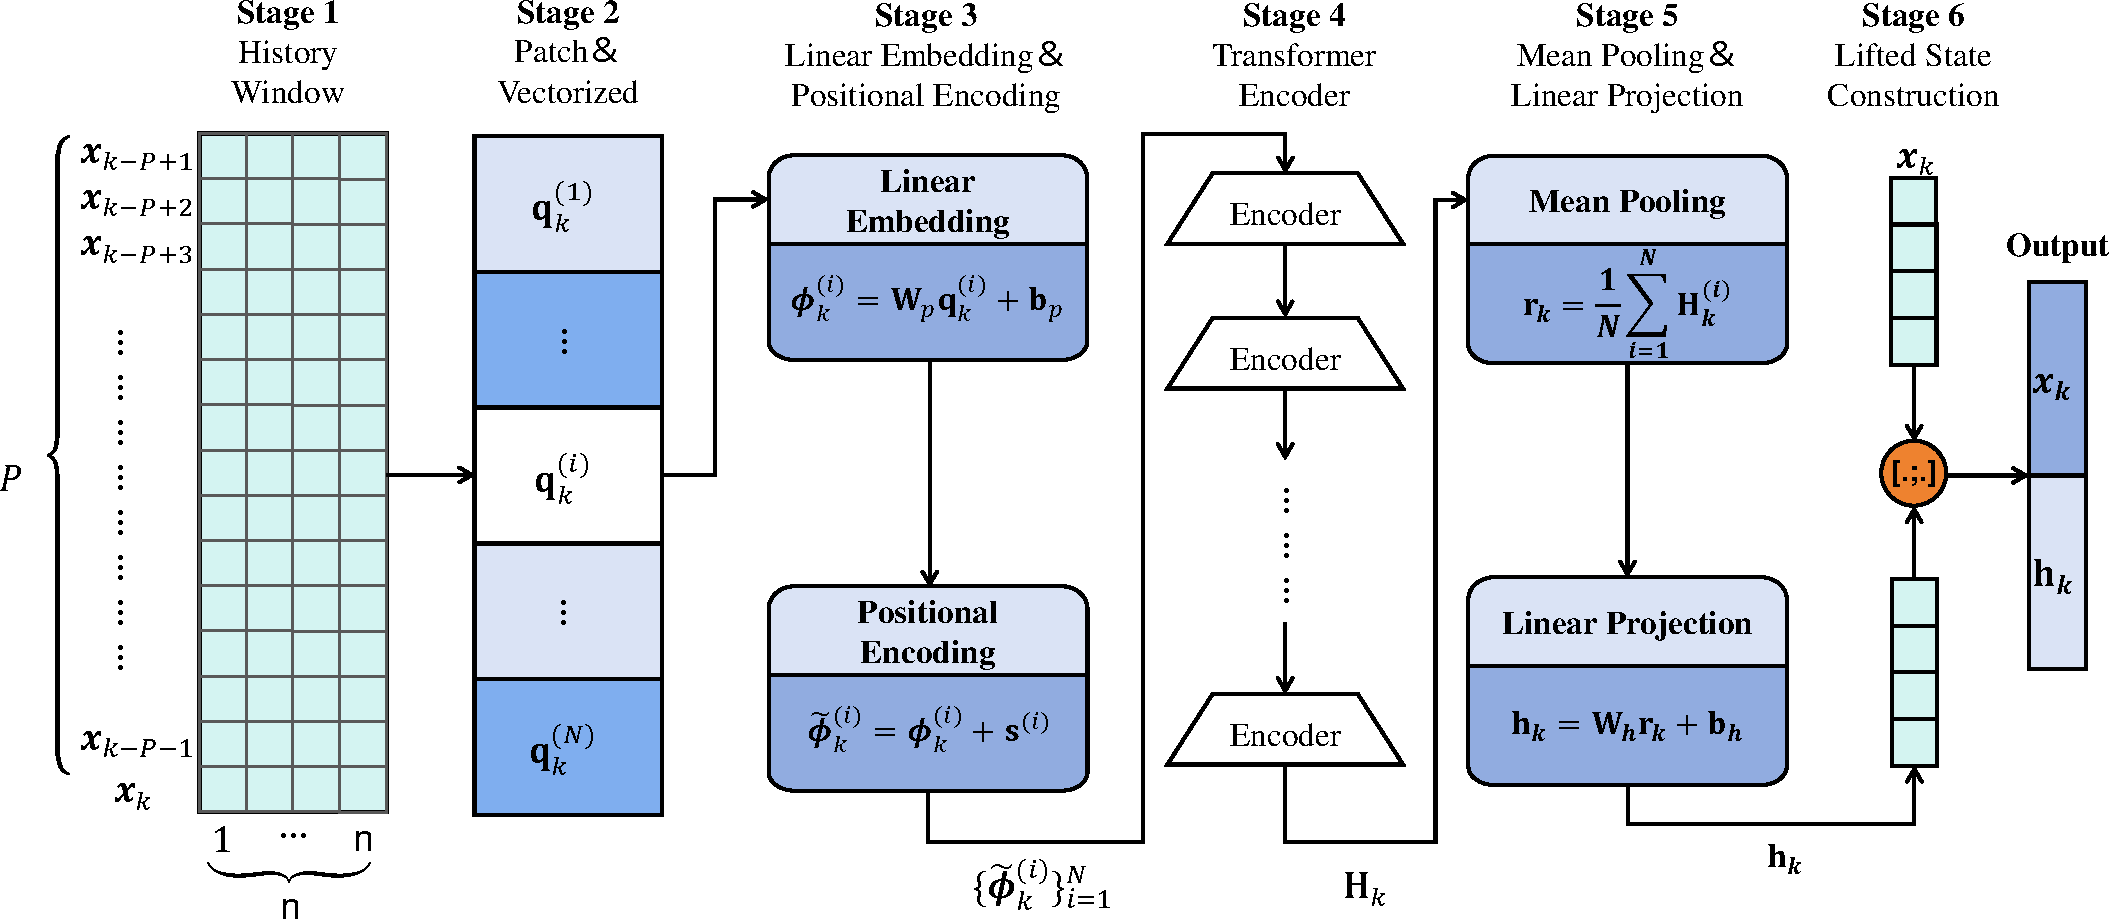
\includegraphics[width=\textwidth]{pictures/Figure1.pdf}
    \caption{Overall prediction pipeline of the proposed
    Transformer-Koopman framework. Given a history window $\mX_k$ and
    the current control input $\vu_k$, the Transformer encoder extracts
    a history feature $\vh_k$, which is concatenated with the current
    state $\vx_k$ to form the lifted state
    $\vz_k = [\vx_k;\,\vh_k] \in \mathbb{R}^d$. The Koopman linear
    dynamics $\hat{\vz}_{k+1} = \mA(\vc_k)\vz_k + \mB\vu_k$ propagate the
    lifted state forward, and the predicted next physical state
    $\hat{\vx}_{k+1} = \mC\hat{\vz}_{k+1}$ is recovered through a
    fixed linear projection.}
    \label{fig:framework}
\end{figure*}

Given the history window $\mX_k \in \mathbb{R}^{P \times n}$, we partition it into $N_p = P/p$ contiguous non-overlapping temporal patches of length $p$, where $p$ is assumed to divide $P$. The $i$th patch is denoted by
\begin{equation}
    \mX_k^{(i)} \in \mathbb{R}^{p \times n}, \qquad i=1,\ldots,N_p.
\end{equation}
Each patch is vectorized as
\begin{equation}
    \vq_k^{(i)} = \mathrm{vec}(\mX_k^{(i)}) \in \mathbb{R}^{pn},
    \label{eq:patch_vec}
\end{equation}
which is then mapped into the Transformer embedding space through a shared linear layer,
\begin{equation}
    \vphi_k^{(i)} = \mW_p \vq_k^{(i)} + \vb_p
    \in \mathbb{R}^{d_{\mathrm{model}}},
    \label{eq:patch_embedding}
\end{equation}
where $\mW_p \in \mathbb{R}^{d_{\mathrm{model}} \times pn}$ and
$\vb_p \in \mathbb{R}^{d_{\mathrm{model}}}$. This patch-based tokenization reduces the sequence length from $P$ to $N_p=P/p$ while preserving local temporal structure within each patch.

The token sequence is augmented with sinusoidal positional encoding \cite{vaswani2017attention} to incorporate temporal order. With $\vp^{(i)}\in\mathbb{R}^{d_{\mathrm{model}}}$ the positional encoding of the $i$th patch, the augmented tokens are
\begin{equation}
    \tilde{\vphi}_k^{(i)} = \vphi_k^{(i)} + \vp^{(i)},
    \label{eq:pos_enc_applied}
\end{equation}
and the resulting token sequence is encoded by an $L$-layer Transformer encoder as
\begin{equation}
    \mH_k = \mathrm{TransformerEncoder}\!\left(
        \{\tilde{\vphi}_k^{(i)}\}_{i=1}^{N_p}
    \right) \in \mathbb{R}^{N_p \times d_{\mathrm{model}}},
    \label{eq:transformer_enc}
\end{equation}
where $L$ is the number of encoder layers and $\mH_k^{(i)} \in \mathbb{R}^{d_{\mathrm{model}}}$ denotes the contextualized representation of the $i$th patch.

We aggregate the patch features by mean pooling to obtain a fixed-dimensional history descriptor:
\begin{equation}
    \vr_k = \frac{1}{N_p}\sum_{i=1}^{N_p} \mH_k^{(i)}
    \in \mathbb{R}^{d_{\mathrm{model}}}.
    \label{eq:pooling}
\end{equation}
After that, the pooled representation is projected to the history-feature space,
\begin{equation}
    \vh_k = \mW_h \vr_k + \vb_h \in \mathbb{R}^{d-n},
    \label{eq:history_feature}
\end{equation}
where $\mW_h \in \mathbb{R}^{(d-n)\times d_{\mathrm{model}}}$ and
$\vb_h \in \mathbb{R}^{d-n}$.

The lifted state is defined as
\begin{equation}
    \vz_k = [\vx_k;\,\vh_k] \in \mathbb{R}^{d},
    \label{eq:lifted_state_form}
\end{equation}
where the first $n$ components of $\vz_k$ are the measured state $\vx_k = h(\vs_k)$ of Section~\ref{subsec:koopman_prelim}, and the remaining $d-n$ components correspond to the temporal features $\vh_k$. This structure allows exact recovery of the \emph{measured} coordinates through the fixed projection
\begin{equation}
    \vx_k = \mC \vz_k, \qquad \mC = [\mI_n\;\mathbf{0}],
    \label{eq:decoder_projection}
\end{equation}
it does not recover components of the physical state $\vs_k$ that the measurement does not observe.

Although the temporal lifting provides different latent representations for different histories, a fixed transition $\mA$ still requires all such history-dependent latent states to evolve under one global linear operator. To relax this additional restriction without discarding the conditional-linear structure, we decompose the transition into a shared nominal component and a structured history-dependent correction.

\begin{definition}[History-Conditioned Low-Rank Koopman Family]
\label{def:hcltk}
Let the history window be $\mX_k$ \eqref{eq:history_window}, and let $\mU^{\mathrm{in}}_k\in\mathbb{R}^{(P-1)\times m}$ denote the input history over the same window \eqref{eq:input_history_problem}. Define the lifted state and the context vector
\begin{equation}
\begin{aligned}
    \vz_k &= g_\theta(\mX_k) = [\vx_k;\,\vh_k],\\
    \vc_k &= C_\phi(\mX_k,\mU^{\mathrm{in}}_k) \in \mathbb{R}^{d_c},
\end{aligned}
    \label{eq:context_vector}
\end{equation}
where $C_\phi$ is a context network and, in the parameterization used here, the two histories of Section~\ref{sec:problem} are concatenated in flattened form into a single input vector of dimension $Pn+(P-1)m$, i.e.\ $C_\phi(\mX_k,\mU^{\mathrm{in}}_k)\equiv\tilde C_\phi\big([\mathrm{vec}\,\mX_k;\mathrm{vec}\,\mU^{\mathrm{in}}_k]\big)$. The lifting map uses the state history to construct a state-preserving representation, whereas the context map additionally uses the past inputs to condition the effective transition on how the current dynamical condition was reached. The model propagates the latent state by
\begin{equation}
    \hat{\vz}^{P}_{k+1} = \mA(\vc_k)\,\vz^{E}_k + \mB\,\vu_k,
    \qquad \vz^{E}_k = g_\theta(\mX_k),
    \label{eq:temporal_dynamics}
\end{equation}
with the \emph{history-conditioned} transition
\begin{equation}
    \mA(\vc) = \mA_0 + \mU\,\mathrm{diag}\big(\gamma_\psi(\vc)\big)\,\mV^\top,
    \qquad
    \mathrm{rank}\big[\mA(\vc)-\mA_0\big] \le r .
    \label{eq:lowrank_A}
\end{equation}
Here $\mA_0 \in \mathbb{R}^{d\times d}$ is the shared nominal transition, $\mU,\mV \in \mathbb{R}^{d\times r}$ are the low-rank factors, $\gamma_\psi:\mathbb{R}^{d_c}\to\mathbb{R}^r$ supplies the context-dependent modulation coefficients, and $\mB \in \mathbb{R}^{d\times m}$ is the input matrix, which is \emph{context-independent} (not context-modulated) and shared across all contexts. The integer $r$ bounds the rank of the correction, $\mathrm{rank}[\mA(\vc)-\mA_0]\le r$, and is a model hyperparameter whose value is reported with the experimental configuration.
\end{definition}

Three remarks follow. First, \eqref{eq:temporal_dynamics} is a prediction rule rather than a Koopman closure of the encoder: the model-propagated latent $\hat{\vz}^{P}_{k+1}$ is not asserted to equal $g_\theta(\mX_{k+1})$, and the two differ by the one-step residual \eqref{eq:modeling_error}, whose propagation under recursive prediction is analyzed in Section~\ref{subsec:rollout}. Second, context dependence is confined to $\mA(\vc)$: the current input enters through the single global matrix $\mB$, so for a fixed context the lifted propagation \eqref{eq:temporal_dynamics} is input-affine in $(\vz_k,\vu_k)$, which is the structure exploited by the local linearization of Section~\ref{sec:control}; over a multi-step prediction horizon the context depends on the predicted history and therefore on preceding control decisions, so the scheduled finite-horizon problem is generally nonlinear. Third, the low-rank term adds a bounded, structured correction to the nominal transition, and all parameters are optimized jointly with the temporal representation, as described next.

% ---------------------------------------------------------
\subsection{Training Procedure}
\label{sec:training}
% ---------------------------------------------------------

The model of Definition~\ref{def:hcltk} has three trainable modules: the lifting encoder with parameters $\theta$ that produce the lifted state $\vz_k$, the context network with parameters $\phi$ that produce $\vc_k=C_\phi(\mX_k,\mU^{\mathrm{in}}_k)$, and the dynamics module, which comprises the nominal transition $\mA_0$, the low-rank factors $\mU,\mV$, the modulation parameters $\psi$, and the input matrix $\mB$. The input matrix $\mB$ is context-independent---a single global matrix shared across all contexts---but it is optimized jointly with the other parameters rather than held frozen. The projection $\mC$ is structurally fixed throughout training, as in Definition~\ref{def:hcltk}. Let $H_R$ denote the training rollout horizon. Each training sample is a segment of $H_R$ future steps cut from a single recorded trajectory, providing an aligned tuple: the history window $\mX_k$, the past-input history $\mU^{\mathrm{in}}_k$, the future inputs $\vu_k,\ldots,\vu_{k+H_R-1}$, and the future measured states $\vx_{k+1},\ldots,\vx_{k+H_R}$ used as prediction targets. Segments do not cross trajectory boundaries.

The history-conditioned transition introduces an additional deployment issue: during one-step training the context is evaluated on measured histories, whereas during recursive prediction it is evaluated on predicted histories, so prediction errors alter the scheduling signal itself. Training therefore proceeds in two stages, which we treat as an optimization schedule rather than a requirement of the model: a nominal one-step initialization, followed by scheduled-rollout fine-tuning of the full history-conditioned family on the \emph{propagated}-latent distribution that arises at deployment.

\textbf{Stage~0 (nominal one-step pretraining).} We initialize the encoder $g_\theta$ and a time-invariant base operator $(\mA_0,\mB)$ by minimizing the one-step physical prediction error over the encoder-generated latent distribution,
\begin{equation}
    \mathcal{L}_{\mathrm{init}}
    =
    \sum_{k}
    \big\|\mC\big(\mA_0\,\vz_k+\mB\,\vu_k\big)-\vx_{k+1}\big\|_2^2,
    \qquad
    \vz_k=g_\theta(\mX_k).
    \label{eq:loss_one_step}
\end{equation}
This stage initializes the temporal encoder and the nominal input-affine predictor using one-step physical-state supervision; it is the only stage optimized exclusively on the encoder-consistent one-step latent distribution, and it corresponds to the fixed (time-invariant) Transformer-Koopman baseline. Because $\mC=[\mI_n\;\mathbf{0}]$ observes only the first $n$ coordinates of the predicted latent, the loss \eqref{eq:loss_one_step} constrains the physical-output rows of $\mA_0$ and $\mB$; the remaining $d-n$ latent rows receive no gradient from this objective and are shaped by the initialization and by the rollout-aware optimization of Stage~1. Fig.~\ref{fig:training_procedure} illustrates the one-step coupling used in this stage.

\begin{definition}[Rollout-Aware Scheduled Objective]
\label{def:rollout_aware}
Starting from the encoder-initialized latent $\vz^{P}_{k}=g_\theta(\mX_k)$, the scheduled rollout is generated for $i=0,\ldots,H_R-1$ by
\begin{equation}
\begin{aligned}
    \vc_{k+i} &= C_\phi(\hat{\mX}_{k+i},\mU^{\mathrm{in}}_{k+i}),\\
    \vz^{P}_{k+i+1} &= \mA(\vc_{k+i})\,\vz^{P}_{k+i} + \mB\,\vu_{k+i},\\
    \hat{\vx}_{k+i+1} &= \mC\,\vz^{P}_{k+i+1},
\end{aligned}
\label{eq:scheduled_rollout}
\end{equation}
where the windows are then shifted by appending the decoded state and the applied input and dropping the oldest entry, $\hat{\mX}_{k+i+1}=\mathrm{shift}(\hat{\mX}_{k+i},\hat{\vx}_{k+i+1})$ and $\mU^{\mathrm{in}}_{k+i+1}=\mathrm{shift}(\mU^{\mathrm{in}}_{k+i},\vu_{k+i})$. The lifting encoder is thus evaluated only at the start of the rollout, while the context is re-scheduled at every step from the history that the predictor itself has produced. With uniform weights $w_i=1/H_R$, the scheduled objective is
\begin{equation}
    \mathcal{L}_R=\sum_k\sum_{i=1}^{H_R} w_i\,\big\|\mC\vz^{P}_{k+i}-\vx_{k+i}\big\|_2^2 .
    \label{eq:loss_rollout}
\end{equation}
\end{definition}

At deployment the transition consumes \emph{propagated} latents $\vz^{P}$, whose distribution differs from the encoder-generated one-step distribution on which Stage~0 is fitted. The rollout objective is an algorithmic training mechanism rather than a theoretical guarantee: no statement in Section~\ref{sec:theory} uses $\mathcal{L}_R$, and Section~\ref{sec:theory} analyzes rollout consistency independently through finite-horizon error propagation.

\textbf{Stage~1 (scheduled-rollout fine-tuning).} We then activate the low-rank context modulation $\mA(\vc_k)=\mA_0+\mU\,\mathrm{diag}(\gamma_\psi(\vc_k))\,\mV^\top$ and jointly refine $\theta$, $\phi$, $\mA_0$, $\mU$, $\mV$, $\gamma_\psi$, and the shared input matrix $\mB$ by minimizing the rollout-aware scheduled objective $\mathcal{L}_R$ of Definition~\ref{def:rollout_aware} \eqref{eq:loss_rollout}, in which the rollout \eqref{eq:scheduled_rollout} propagates the latent and \emph{re-schedules} the context from the history that the predictor itself has produced (Section~\ref{subsec:rollout}). Only the projection $\mC$ is structurally fixed. The horizon and weights used in this work are reported with the experimental configuration.

Minimizing $\mathcal{L}_R$ trains the operator on the propagated-latent distribution that arises at deployment, rather than on the encoder-generated one-step distribution; this is the rollout mismatch between encoder-initialized and recursively propagated latent states analyzed in Section~\ref{subsec:rollout}.

The modulation is parameterized with a total absolute budget that limits the magnitude of the context-dependent correction: the columns of $\mU$ and $\mV$ are reparameterized to unit norm, and $\gamma_\psi$ is reparameterized so that its components obey $\sum_{i=1}^{r}|\gamma_{\psi,i}(\vc)|\le g_{\max}$ for all $\vc$, their signs being unconstrained. Both are structural reparameterizations rather than training penalties. Writing $\mA(\vc)-\mA_0=\sum_{i=1}^{r}\gamma_{\psi,i}(\vc)\,\mU_{:,i}\mV_{:,i}^{\top}$ with unit-norm columns $\|\mU_{:,i}\|_2=\|\mV_{:,i}\|_2=1$, the triangle inequality together with $\|\mU_{:,i}\mV_{:,i}^{\top}\|_2=1$ gives
\begin{equation}
    \|\mA(\vc)-\mA_0\|_2
    \le \sum_{i=1}^{r}\big|\gamma_{\psi,i}(\vc)\big|
    \le g_{\max},
    \label{eq:correction_bound}
\end{equation}
uniformly in $\vc$. This bound controls the size of the correction only: it does not imply that $\mA(\vc)$ is well-conditioned, that $\|\mA(\vc)\|_2<1$ or $\rho(\mA(\vc))<1$, or that the scheduled products $\mA_{k+H-1}\cdots\mA_k$ contract, and no stability property is claimed on this basis (Section~\ref{sec:theory}).

The complete procedure is summarized in Algorithm~\ref{alg:training}.

\begin{algorithm}[!t]
\caption{Transformer-Koopman Training Algorithm}
\label{alg:training}
\begin{algorithmic}[1]

\STATE \textbf{Input:} Trajectory dataset $\mathcal{D}$ \eqref{eq:trajectory_dataset}
\STATE History length $P$; patch length $p$; lifted dimension $d$; rank $r$; rollout horizon $H_R$
\STATE Rollout weights $w_1,\ldots,w_{H_R}$; epochs $E_0$ (nominal pretraining), $E_1$ (scheduled-rollout fine-tuning)

\STATE \textbf{Output:} Lifting encoder $\theta^{*}$; context $\phi^{*}$; transition parameters $\mA_0^{*},\mU^{*},\mV^{*},\gamma_\psi^{*}$; input matrix $\mB^{*}$

\STATE \textbf{Stage~0 (nominal one-step pretraining):}
Initialize $\theta$ and $(\mA_0,\mB)$; for $E_0$ epochs, minimize the one-step loss \eqref{eq:loss_one_step} over $(\theta,\mA_0,\mB)$.

\vspace{2pt}

\STATE \textbf{Stage~1 (scheduled-rollout fine-tuning):}
Activate $\mA(\vc)=\mA_0+\mU\,\mathrm{diag}(\gamma_\psi(\vc))\,\mV^\top$ and initialize $(\phi,\mU,\mV,\psi)$; keep only $\mC$ structurally fixed.
\FOR{epoch $\ell = 1$ \TO $E_1$}
    \FOR{each mini-batch $\mathcal{S}$ of length-$H_R$ segments drawn from $\mathcal{D}$}
        \STATE Initialize the rollout at $\vz^{P}_{k}=g_\theta(\mX_k)$.
        \FOR{$i=0$ \TO $H_R-1$}
            \STATE Re-schedule the context $\vc_{k+i}=C_\phi(\hat{\mX}_{k+i},\mU^{\mathrm{in}}_{k+i})$ from the rolled-out history.
            \STATE Propagate $\vz^{P}_{k+i+1}=\mA(\vc_{k+i})\vz^{P}_{k+i}+\mB\vu_{k+i}$ and shift the windows using $\hat{\vx}_{k+i+1}=\mC\vz^{P}_{k+i+1}$.
        \ENDFOR
        \STATE Form the scheduled objective $\mathcal{L}_R$ \eqref{eq:loss_rollout}.
        \STATE Update $(\theta,\phi,\mA_0,\mU,\mV,\gamma_\psi,\mB)$ by backpropagation through the rollout.
    \ENDFOR
\ENDFOR

\RETURN $\theta^{*},\phi^{*},\mA_0^{*},\mU^{*},\mV^{*},\gamma_\psi^{*},\mB^{*}$

\end{algorithmic}
\end{algorithm}

\begin{figure*}[!t]
    \centering
    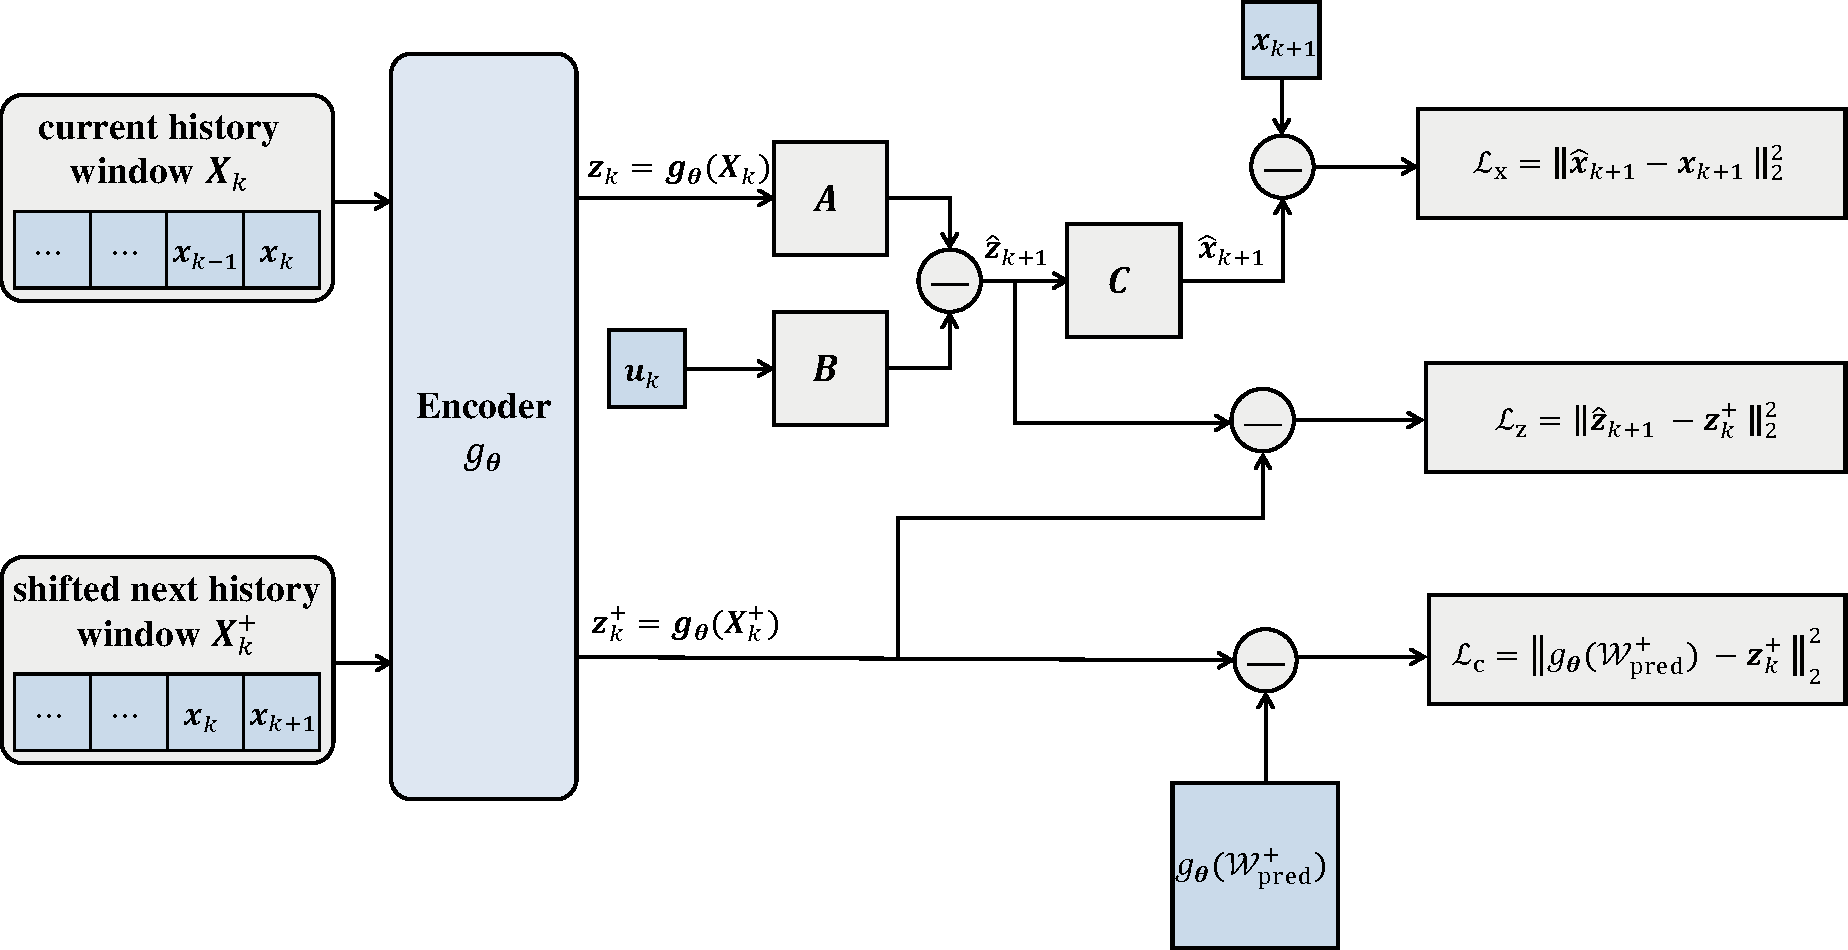
\includegraphics[width=0.95\textwidth]{pictures/Figure2.pdf}
    \caption{One-step lifting and prediction (nominal pretraining, Stage~0). The
    history window $\mX_k$ is encoded by $g_\theta$ to produce the lifted
    state $\vz_k$, and the time-invariant base operator $(\mA_0,\mB)$
    produces the one-step prediction $\hat{\vz}_{k+1}=\mA_0\vz_k+\mB\vu_k$,
    from which $\hat{\vx}_{k+1}$ is recovered via $\mC$. Stage-0 training is
    supervised only through the decoded physical state, by the one-step loss
    \eqref{eq:loss_one_step}; the shifted window $\mX_k^{+}$ indicates the
    sliding-window convention over the dataset and does not enter the Stage-0
    objective. Stage~1 replaces $\mA_0$ by the history-conditioned
    $\mA(\vc)$ and jointly refines the full model on the rollout-aware
    scheduled objective (Algorithm~\ref{alg:training}).}
    \label{fig:training_procedure}
\end{figure*}


% =========================================================
\section{Finite-Horizon Consistency Analysis}
\label{sec:theory}
% =========================================================

In this section, we analyze the internal finite-history predictor of Section~\ref{sec:methodology} and its finite-horizon error propagation. Section~\ref{subsec:rollout} bounds the inconsistency that arises when the latent state is propagated recursively instead of being re-encoded, and Section~\ref{subsec:fh_bound} bounds the finite-horizon prediction error of the learned augmented predictor against a recorded reference sequence. All statements are conditional on the regularity assumptions stated below and concern the predictor itself; the scope remark at the end of the section states what is \emph{not} claimed.

Because the lifted state is a function of a finite window, the predictor can be recast as a first-order system on an augmented state. Define
\begin{equation}
    \vxi_k = \mathrm{col}\big(\mathrm{vec}\,\mX_k,\,\mathrm{vec}\,\mU^{\mathrm{in}}_k,\,\vz_k\big)
    \in \mathbb{R}^{Pn+(P-1)m+d},
    \label{eq:augmented_state}
\end{equation}
and consider the predictor's own rollout, in which the newest fed-back state is its decoded output $\hat{\vx}_{k+1}=\mC\vz_{k+1}$. The window update is then a deterministic shift: append the decoded state and the applied input, and drop the oldest entry. Since $\mX_k$ and $\mU^{\mathrm{in}}_k$ are sub-blocks of $\vxi_k$, every argument of that update is a function of $(\vxi_k,\vu_k)$ alone, so composing the shift, the context map, the transition, and the decoder yields a single deterministic map
\begin{equation}
    \vxi_{k+1} = \mF_\Theta(\vxi_k, \vu_k).
    \label{eq:augmented_map}
\end{equation}
This construction describes the predictor's internal rollout only. If a true measurement $\vx_{k+1}$ is fed back instead, the update also depends on an exogenous quantity and is not a function of $\vxi_k$ alone; and nothing here asserts that the finite measured history Markovizes the physical system \eqref{eq:nonlinear_system}.

\subsection{Latent Rollout Inconsistency and Its Propagation}
\label{subsec:rollout}

We now characterize the discrepancy that arises when the latent state is propagated recursively instead of being re-encoded at every step.

\begin{definition}[Latent Rollout Inconsistency]
\label{def:rollout}
Let $\hat{\mX}_{k+i}$ be the history produced by the predictor's own rollout and let $\vc_{k+i}=C_\phi(\hat{\mX}_{k+i},\mU^{\mathrm{in}}_{k+i})$ denote the scheduled context re-computed from it. Define the encoder-consistent latent and the propagated latent,
\begin{equation}
    \vz^{E}_{k+i} = g_\theta(\hat{\mX}_{k+i}), \qquad
    \vz^{P}_{k+i+1} = \mA(\vc_{k+i})\vz^{P}_{k+i} + \mB\vu_{k+i},
\end{equation}
and the normalized rollout defect
\begin{equation}
    d_{\mathcal{M},k+i} = \frac{\big\|\vz^{P}_{k+i}-\vz^{E}_{k+i}\big\|_2}{\big\|\vz^{E}_{k+i}\big\|_2+\epsilon_0},
    \label{eq:defect}
\end{equation}
with $\epsilon_0=10^{-6}$ a fixed numerical floor. We also use the absolute defect $d^{\mathrm{abs}}_{k+i}=\|\vz^{P}_{k+i}-\vz^{E}_{k+i}\|_2$, which is the quantity for which Proposition~\ref{prop:propagation} provides an upper bound.
\end{definition}

Two properties of this defect are worth stating explicitly. First, because $\vz=[\vx;\vh]$ is state-preserving and the newest entry of $\hat{\mX}_{k+i}$ is the decoded state $\mC\vz^{P}_{k+i}$, the propagated and the encoder-consistent latents share their first $n$ coordinates, $\mC(\vz^{P}_{k+i}-\vz^{E}_{k+i})=\mathbf{0}$; the defect therefore measures the inconsistency of the remaining $d-n$ hidden lifted coordinates rather than a physical multi-step prediction error. Those hidden coordinates still affect future decoded predictions through $\mA(\vc)$, which is why this inconsistency matters. Second, evaluating $\vz^{E}_{k+i}$ requires an additional encoder pass on the predicted history. That pass is an offline diagnostic used to characterize the mechanism; it is not part of the online rollout, in which the context is re-scheduled without re-running the encoder inside the horizon (Section~\ref{sec:control}).

\begin{proposition}[Latent Rollout Error Propagation]
\label{prop:propagation}
Let $\vz^{P}_{k}$ denote the recursively propagated latent state and $\vz^{E}_{k}=g_\theta(\hat{\mX}_k)$ the encoder-consistent latent state, and let $d_k\equiv d^{\mathrm{abs}}_k=\|\vz^{P}_k-\vz^{E}_k\|_2$. Define the encoder-consistent one-step defect
\begin{equation}
    \epsilon_k = \big\|\mA(\vc_k)\vz^{E}_k + \mB\vu_k - \vz^{E}_{k+1}\big\|_2 .
\end{equation}
Then $d_{k+1}\le\|\mA(\vc_k)\|_2\,d_k+\epsilon_k$, and for any horizon $H$,
\begin{equation}
    \begin{aligned}
    d_{k+H}\le{}&
    \big\|\mA_{k+H-1}\cdots\mA_{k}\big\|_2\,d_k \\
    &+\sum_{i=0}^{H-1}\big\|\mA_{k+H-1}\cdots\mA_{k+i+1}\big\|_2\,\epsilon_{k+i},
    \end{aligned}
    \label{eq:prop_bound}
\end{equation}
where $\mA_{k+j}=\mA(\vc_{k+j})$ is the transition at the scheduled context $\vc_{k+j}=C_\phi(\hat{\mX}_{k+j},\mU^{\mathrm{in}}_{k+j})$ along the same rollout. If the rollout starts from an encoder-consistent latent ($\vz^{P}_k=\vz^{E}_k$, hence $d_k=0$), the first term vanishes and the bound reduces to the second sum alone. The bound is a trajectory-wise recursion: both $\epsilon_k$ and the transition matrices $\mA_{k+j}$ are evaluated along the same rollout, so they depend on the realized trajectory rather than being a priori constants.
\end{proposition}

\begin{proof}
Let $\ve_k=\vz^{P}_k-\vz^{E}_k$ denote the latent error. Subtracting the encoder-consistent update from the propagation rule $\vz^{P}_{k+1}=\mA(\vc_k)\vz^{P}_k+\mB\vu_k$ gives the linear recursion
\begin{equation*}
    \ve_{k+1}=\mA(\vc_k)\ve_k+\vr^{z}_k,
    \qquad
    \vr^{z}_k=\mA(\vc_k)\vz^{E}_k+\mB\vu_k-\vz^{E}_{k+1},
\end{equation*}
where $\|\vr^{z}_k\|_2=\epsilon_k$. Taking norms and using the triangle inequality and submultiplicativity yields the one-step bound $d_{k+1}\le\|\mA(\vc_k)\|_2\,d_k+\epsilon_k$. Unrolling the recursion over $H$ steps gives
\begin{align*}
    \ve_{k+H}
    &=\mA_{k+H-1}\cdots\mA_{k}\,\ve_k \\
    &\quad+\sum_{i=0}^{H-1}\mA_{k+H-1}\cdots\mA_{k+i+1}\,\vr^{z}_{k+i},
\end{align*}
and taking norms, with $\|\ve_k\|_2=d_k$ and $\|\vr^{z}_{k+i}\|_2=\epsilon_{k+i}$, gives \eqref{eq:prop_bound} (the empty product at $i=H-1$ is the identity). Since $\|\mA_{k+H-1}\cdots\mA_{k}\|_2\le\prod_{j=0}^{H-1}\|\mA_{k+j}\|_2$, this matrix-product form is at least as tight as the product-of-norms form.
\end{proof}

Equation~\eqref{eq:prop_bound} shows that the long-horizon inconsistency is governed by two factors: the local one-step defect $\epsilon_k$ and the \emph{amplification of the time-varying transition products}.

\begin{remark}[Why spectral stabilization is insufficient]
\label{rem:spectral}
Enforcing $\rho(\mA(\vc_k))<1$ for all $k$ does \emph{not} imply a uniform contraction of the time-varying products:
\begin{equation}
    \rho(\mA_k)<1\ \ \forall k \ \ \not\Rightarrow\ \ \|\mA_{k+H-1}\cdots\mA_k\|_2\le c<1 ,
\end{equation}
which is the classical spectral-radius/joint-spectral-radius gap for non-commuting matrices \cite{daubechies1992sets, rota1960joint, jungers2009joint}. A bound on $\rho(\mA(\vc))$ therefore does not by itself control the amplification of the scheduled products that appears in \eqref{eq:prop_bound}.
\end{remark}

\subsection{Finite-Horizon Prediction Error Bound}
\label{subsec:fh_bound}

To state the bound we compare the learned predictor with a \emph{reference augmented sequence} built directly from the recorded observations, rather than postulating a deterministic reference transition for the plant. Let
\begin{equation}
    \vxi^{\star}_k=\mathrm{col}\big(\mathrm{vec}\,\mX_k,\,\mathrm{vec}\,\mU^{\mathrm{in}}_k,\,g_\theta(\mX_k)\big)
    \label{eq:true_augmented}
\end{equation}
denote the reference augmented state built from the true observations and the encoder-consistent latent, and let $\vxi^{\star}_{k+1}$ be its successor along the recorded trajectory. The reference sequence consists of measured quantities; no deterministic reference map is assumed to generate it, so the finite observed history is never asserted to Markovize the underlying plant. The learned augmented transition $\mF_\Theta$ is the map \eqref{eq:augmented_map}, which propagates the latent and feeds back the decoded output $\hat{\vx}=\mC\vz^{P}$. We therefore measure the learned model by its one-step discrepancy on the reference sequence,
\begin{equation}
    \delta^{\star}_k=\big\|\vxi^{\star}_{k+1}-\mF_\Theta(\vxi^{\star}_k,\vu_k)\big\|_2 .
    \label{eq:ref_discrepancy}
\end{equation}
This quantity bundles the physical modeling error, the finite-history truncation error, the learned transition error, and the difference between the encoder-consistent and the propagated latent updates.

On the recorded sequence we also define the one-step modeling residual at the encoder-consistent latent,
\begin{equation}
    \vw_k = \vz^{E}_{k+1} - \big(\mA(\vc_k)\vz^{E}_k + \mB \vu_k\big),
    \qquad \vz^{E}_{k}=g_\theta(\mX_k),
    \label{eq:modeling_error}
\end{equation}
which measures one-step data consistency on recorded histories. It is not an independent error quantity: because the history and input shifts are exact and the encoder is state-preserving, $\mC\vz^{E}_{k+1}=\vx_{k+1}$, and the augmented one-step reference discrepancy \eqref{eq:ref_discrepancy} reduces to
\begin{equation}
    (\delta^{\star}_k)^2=\|\vw_k\|_2^2+\|\mC\vw_k\|_2^2 ,
    \qquad
    \|\vw_k\|_2\le\delta^{\star}_k\le\sqrt{2}\,\|\vw_k\|_2 ,
    \label{eq:w_delta_relation}
\end{equation}
so $\delta^{\star}_k$ and $\vw_k$ are two views of the same one-step discrepancy on recorded data. This identity uses the history shift, the fixed projection $\mC=[\mI_n\;\mathbf{0}]$, and the re-encoding of the next recorded state adopted here; it is not an unconditional relation for arbitrary feedback structures. The defect $\epsilon_k$ of Proposition~\ref{prop:propagation}, by contrast, is evaluated on histories generated by the predictor itself and cannot be replaced by statistics of $\vw_k$.

\begin{assumption}[Operating-set reference discrepancy]
\label{as:mismatch}
There exist a compact \emph{operating set} $\Omega\subset\mathbb{R}^{Pn+(P-1)m+d}\times\mathbb{R}^m$, i.e.\ a set of augmented state--input pairs $(\vxi,\vu)$, and a finite constant $\epsilon\ge0$ such that, along the reference sequence and at every step of the considered horizon, the one-step reference discrepancy \eqref{eq:ref_discrepancy} satisfies $\delta^{\star}_k\le\epsilon$, equivalently
\begin{equation}
    \big\|\vxi^{\star}_{k+1}-\mF_\Theta(\vxi^{\star}_k,\vu_k)\big\|_2\le\epsilon .
    \label{eq:as_mismatch}
\end{equation}
We additionally require that the reference and predicted trajectories remain in $\Omega$ over the considered horizon; this condition is used explicitly in Theorem~\ref{thm:fh}.
\end{assumption}

\begin{assumption}[Lipschitz continuity of the learned transition]
\label{as:lipschitz}
There exists a finite constant $\mLf$ such that
\begin{equation}
    \|\mF_\Theta(\vxi_1,\vu)-\mF_\Theta(\vxi_2,\vu)\|_2\le \mLf\|\vxi_1-\vxi_2\|_2
    \label{eq:as_lipschitz}
\end{equation}
for all $(\vxi_1,\vu),(\vxi_2,\vu)\in\Omega$.
No contraction is assumed: $\mLf$ need not be smaller than one. The bound holds on $\Omega$ whenever the context map $C_\phi$, the modulation $\gamma_\psi$, and the map $\vc\mapsto\mA(\vc)$ are Lipschitz there and the lifted state stays bounded; we take these as standing regularity conditions on the learned components. These conditions concern the functions that the recursion \eqref{eq:augmented_map} actually composes---the context map, the modulation, the low-rank transition, the affine latent update and decoding, and the exact window shift---and not the lifting encoder: $g_\theta$ is evaluated only to initialize the rollout, and is not re-evaluated inside $\mF_\Theta$. In the parameterization used here the context map and the modulation are composed of affine layers and smooth activations, so on a bounded operating set these conditions are met.
\end{assumption}

\begin{theorem}[Finite-Horizon Prediction Error Bound]
\label{thm:fh}
For a common prescribed input sequence $\{\vu_k,\ldots,\vu_{k+H-1}\}$, suppose that the reference and predicted trajectories remain in the operating set $\Omega$ over the horizon $H$. Under Assumptions~\ref{as:mismatch} and \ref{as:lipschitz}, and with $e_k=\vxi^{\star}_k-\hat{\vxi}_k$,
\begin{equation}
    \|e_{k+H}\|_2 \le \mLf^{H}\|e_k\|_2+\sum_{i=0}^{H-1}\mLf^{H-1-i}\,\delta^{\star}_{k+i}.
    \label{eq:fh_bound}
\end{equation}
If in addition the reference discrepancy is uniformly bounded by $\epsilon$ as in Assumption~\ref{as:mismatch}, then
\begin{equation}
    \|e_{k+H}\|_2 \le \mLf^{H}\|e_k\|_2+\epsilon\sum_{j=0}^{H-1}\mLf^{j}.
    \label{eq:fh_bound_uniform}
\end{equation}
If the horizon is initialized from the same measured history and the corresponding encoder-consistent latent state, i.e. $\hat{\mX}_k=\mX_k$ and $\vz^{P}_k=g_\theta(\mX_k)$, then $e_k=0$ and $\|e_{k+H}\|_2\le\epsilon\sum_{j=0}^{H-1}\mLf^{j}$. The bound compares the learned predictor with the recorded reference trajectory under a \emph{common} input sequence; it is not a closed-loop tracking-error or robustness statement. Here $\epsilon$ is the uniform bound of Assumption~\ref{as:mismatch}.
\end{theorem}

\begin{proof}
For one step, using the recorded successor $\vxi^{\star}_{k+1}$,
\begin{align*}
    \|e_{k+1}\|_2
    &=\big\|\vxi^{\star}_{k+1}-\mF_\Theta(\hat{\vxi}_k,\vu_k)\big\|_2 \\
    &\le\big\|\vxi^{\star}_{k+1}-\mF_\Theta(\vxi^{\star}_k,\vu_k)\big\|_2 \\
    &\quad+\big\|\mF_\Theta(\vxi^{\star}_k,\vu_k)-\mF_\Theta(\hat{\vxi}_k,\vu_k)\big\|_2 \\
    &\le\delta^{\star}_k+\mLf\|e_k\|_2 ,
\end{align*}
by \eqref{eq:ref_discrepancy} and Assumption~\ref{as:lipschitz}, which applies at every step because the trajectories remain in $\Omega$ over the horizon. Unrolling the recursion yields \eqref{eq:fh_bound}; bounding each $\delta^{\star}_{k+i}$ by $\epsilon$ yields \eqref{eq:fh_bound_uniform}.
\end{proof}

\begin{remark}[How to read these bounds]
\label{rem:eps_vs_epsk}
Equation~\eqref{eq:fh_bound} is a conditional finite-horizon relation between two trajectories driven by the same input sequence, not a numerical certificate. The quantities $\epsilon$, $\epsilon_k$ and $\vw_k$ are defined on different trajectories and are not interchangeable, and the regularity constants of Assumptions~\ref{as:mismatch} and \ref{as:lipschitz} are properties of the operating set $\Omega$ rather than of any validation sample. The bound concerns the rolled-out predictor under a common input sequence: when $\mLf>1$ it grows geometrically with $H$, and it is neither a closed-loop tracking-error statement nor a stability result.
\end{remark}

The bound above concerns the augmented state, and the physical coordinates are a sub-vector of it. Both the current physical state $\vx_{k+H}$ and the predictor's decoded feedback $\hat{\vx}_{k+H}=\mC\vz^{P}_{k+H}$ occupy the last $n$ coordinates of the history block of the respective augmented states, so their difference is a coordinate sub-vector of $\hat{\vxi}_{k+H}-\vxi^{\star}_{k+H}$. Since a coordinate sub-vector has at most the norm of the full vector, Theorem~\ref{thm:fh} gives directly, with no additional assumption,
\begin{equation}
    \|\hat{\vx}_{k+H}-\vx_{k+H}\|_2
    \le \mLf^{H}\|e_k\|_2+\sum_{i=0}^{H-1}\mLf^{H-1-i}\,\delta^{\star}_{k+i}.
    \label{eq:cor_physical}
\end{equation}

\begin{remark}[Scope of the analysis]
\label{subsec:scope}
The analysis is finite-horizon and concerns the consistency of the learned predictor and the propagation of its prediction error; the local linearization accuracy of the RTI step is treated separately in Section~\ref{sec:control}. It does not establish global closed-loop stability, a common Lyapunov function, terminal invariant sets, or recursive feasibility under learned uncertainty. The regularity constants used for the empirical assessment are operating-region diagnostics rather than global certificates, all bounds concern the rolled-out latent predictor rather than true-plant tracking error, and $\mA(\vc)$ is a latent linearization parameterization rather than an exact Koopman invariant-subspace operator.
\end{remark}

% =========================================================
\section{Real-Time Predictive Control}
\label{sec:control}
% =========================================================

In this section, we embed the learned history-conditioned predictor into a receding-horizon controller. The prediction rollout propagates the lifted state while updating the scheduling context from decoded state histories, and the optimization is approximated by one real-time-iteration (RTI) step per control update \cite{diehl2005realtime, gros2020rti} to reduce the online computation of each update; whether a given sampling constraint is met is an empirical question.

\subsection{History-Consistent Scheduled Prediction}

At control instant $k$ the controller is initialized from the measured history and predicts over a horizon $N$ according to
\begin{align}
    \hat{\mX}_{k|k}&=\mX_k,\qquad \mU^{\mathrm{in}}_{k|k}=\mU^{\mathrm{in}}_k,\notag\\
    \vz_{k|k}&=g_\theta(\mX_k),\notag\\
    \vc_{k+i|k}&=C_\phi\big(\hat{\mX}_{k+i|k},\mU^{\mathrm{in}}_{k+i|k}\big),\notag\\
    \vz_{k+i+1|k}&=\mA(\vc_{k+i|k})\,\vz_{k+i|k}+\mB\,\vu_{k+i|k},\notag\\
    \hat{\vx}_{k+i+1|k}&=\mC\,\vz_{k+i+1|k},\notag\\
    \hat{\mX}_{k+i+1|k}&=\mathrm{shift}\big(\hat{\mX}_{k+i|k},\hat{\vx}_{k+i+1|k}\big),\notag\\
    \mU^{\mathrm{in}}_{k+i+1|k}&=\mathrm{shift}\big(\mU^{\mathrm{in}}_{k+i|k},\vu_{k+i|k}\big),
    \label{eq:scheduled_predictor}
\end{align}
where $i=0,\ldots,N-1$ and $i|k$ denotes prediction step $i$ from control instant $k$. This is the same \emph{context-re-scheduled, latent-propagated} recursion as the training rollout \eqref{eq:scheduled_rollout}: the lifting encoder is evaluated once per control instant, at the start of the horizon, and the context is re-scheduled at every step from the decoded history rather than re-encoded. At the next sampling instant the controller is re-initialized from the newly measured history, which does not re-run the encoder inside the horizon. The alternative---re-encoding the history at every prediction stage (RTI-RE)---requires one additional encoder evaluation per prediction stage; whether that additional evaluation improves accuracy is an empirical question left to the experiments.

\subsection{One-Iteration RTI}

Writing $\mUs=\mathrm{col}(\vu_{k|k},\ldots,\vu_{k+N-1|k})\in\mathbb{R}^{Nm}$ for the stacked input sequence over the horizon, we solve the receding-horizon problem
\begin{equation}
\begin{aligned}
    \min_{\mUs}\ \ &\sum_{i=1}^{N}\big\|\hat{\vx}_{k+i|k}-\vx^{\mathrm{ref}}_{k+i}\big\|_{\mQ}^2\\
    &+\sum_{i=0}^{N-1}\Big(\big\|\vu_{k+i|k}\big\|_{\mR}^2+\big\|\vu_{k+i|k}-\vu_{k+i-1|k}\big\|_{\mS}^2\Big),
\end{aligned}
    \label{eq:mpc_cost}
\end{equation}
subject to the componentwise input box $\vu_{\min}\le\vu_{k+i|k}\le\vu_{\max}$. In the input-rate term the predecessor is the previously \emph{applied} input, $\vu_{k-1|k}=\vu^{\mathrm{app}}_{k-1}$, which is a known constant rather than a decision variable, and $\mQ,\mR,\mS$ are positive semidefinite weights. Because the scheduled context depends on the predicted history, the predicted states in \eqref{eq:mpc_cost} depend on the whole input sequence, so this problem is generally nonlinear and is not solved as a convex program; it is handled locally, as follows. No terminal cost, terminal set, state constraint, or robust tube is imposed, and none is claimed below.

One RTI step per sampling instant for \eqref{eq:mpc_cost} consists of: (i) warm-starting the input sequence from the previous solution shifted by one step; (ii) rolling out the nominal trajectory \eqref{eq:scheduled_predictor} at that sequence; (iii) evaluating, along the nominal trajectory, the sensitivities
\begin{equation}
\begin{aligned}
    \mF_i&=\frac{\partial\mF_\Theta}{\partial\vxi}\Big|_{(\bar\vxi_i,\bar\vu_i)},
    \qquad
    \mG_i=\frac{\partial\mF_\Theta}{\partial\vu}\Big|_{(\bar\vxi_i,\bar\vu_i)},\\
    \delta\vxi_{i+1}&=\mF_i\,\delta\vxi_i+\mG_i\,\delta\vu_i ,
\end{aligned}
    \label{eq:rti_linearization}
\end{equation}
and composing them along the rollout into the sensitivity of the predicted outputs to the \emph{whole} input sequence; this retains the dependence of every scheduled context on the inputs applied before it, and does not treat $\mA(\vc_i)$ as a fixed matrix; (iv) solving one local quadratic subproblem in the increments $\delta\mUs$ around the nominal value $\bar{\mUs}$,
\begin{equation}
\begin{aligned}
    \min_{\delta\mUs}\ \ &\tfrac12\,\delta\mUs^{\top}\mH_{\mathrm{RTI}}\,\delta\mUs
        +\mathbf{g}_{\mathrm{RTI}}^{\top}\delta\mUs ,\\
    \text{s.t.}\ \ &\vu_{\min}-\bar{\mUs}\le\delta\mUs\le\vu_{\max}-\bar{\mUs},
\end{aligned}
    \label{eq:rti_qp}
\end{equation}
in which $\mH_{\mathrm{RTI}}$ and $\mathbf{g}_{\mathrm{RTI}}$ are determined by the weights $\mQ,\mR,\mS$, the nominal prediction, and the composed sensitivities of step (iii); $\mH_{\mathrm{RTI}}$ is symmetric and positive semidefinite for the stated weights but need not be positive definite, and the subproblem is solved numerically rather than in closed form; and (v) applying only the first input, $\vu^{\mathrm{app}}_k=\bar\vu_k+\delta\vu_k$.

Because the bounds act on the increments, $\delta\vu=\mathbf{0}$ is feasible for this subproblem whenever the warm-start nominal input lies inside the box. This is feasibility of the linearized subproblem only: it does not imply recursive feasibility of the nonlinear problem, and no claim is made here of strict convexity, of a unique minimizer, of exact minimization, or of global SQP convergence. The practical adequacy of a single iteration is assessed empirically against a matched exact scheduled NMPC oracle in Section~\ref{sec:experiments}.

The accuracy of step (iii) is characterized by the local second-order remainder of the augmented map. Treating $\mF_\Theta$ as a function of the joint variable $\eta=\mathrm{col}(\vxi,\vu)$, let $\bar\eta_i=\mathrm{col}(\bar\vxi_i,\bar\vu_i)$ and $\delta\eta_i=\mathrm{col}(\delta\vxi_i,\delta\vu_i)$ denote the nominal point and the joint perturbation.

\begin{assumption}[Local second-order regularity of the augmented map]
\label{as:hessian}
The nominal point $\bar\eta_i$ and the perturbation segment $\{\bar\eta_i+s\,\delta\eta_i:\ s\in[0,1]\}$ lie in a common region on which $\mF_\Theta$ is twice continuously differentiable, and on that segment the second derivative is bounded by $\|\mathrm{D}^2\mF_\Theta\|_2\le\mMF$, where $\|\cdot\|_2$ denotes the operator norm of the second-derivative bilinear form. The remainder below is used only for perturbations whose segment lies within one such region: it is a local statement, and the same estimate is not asserted for a segment that crosses a boundary on which $\mF_\Theta$ is not twice differentiable.
\end{assumption}

Under Assumption~\ref{as:hessian} the expansion
\begin{equation}
\begin{aligned}
    \mF_\Theta(\bar\eta_i+\delta\eta_i)&=\mF_\Theta(\bar\eta_i)+\mathrm{D}\mF_\Theta(\bar\eta_i)\,\delta\eta_i+\mathcal{R}_i,\\
    \mathrm{D}\mF_\Theta(\bar\eta_i)\,\delta\eta_i&=\mF_i\,\delta\vxi_i+\mG_i\,\delta\vu_i,
\end{aligned}
\label{eq:taylor_expansion}
\end{equation}
has the integral remainder
\begin{equation}
    \mathcal{R}_i=\int_0^1(1-s)\,\mathrm{D}^2\mF_\Theta\big(\bar\eta_i+s\delta\eta_i\big)\big[\delta\eta_i,\delta\eta_i\big]\,\mathrm{d}s ,
    \label{eq:taylor_remainder}
\end{equation}
where $\mathrm{D}^2\mF_\Theta[\cdot,\cdot]$ is the second-derivative bilinear form, and bounding the norm of the integral by the integral of the norm gives
\begin{equation}
    \|\mathcal{R}_i\|_2 \le \frac{\mMF}{2}\big\|\delta\eta_i\big\|_2^2 .
    \label{eq:rti_remainder}
\end{equation}
This bounds the model error of the local linearization used in step (iii), and it is local to the region of Assumption~\ref{as:hessian}: it is a property of the linearization itself, and it neither bounds the performance of a single RTI iteration nor establishes SQP convergence, recursive feasibility, or closed-loop stability.

% =========================================================
\section{Experiments}
\label{sec:experiments}
% =========================================================

This section reports a training-schedule ablation of the history-conditioned predictor, followed by the empirical diagnostics that assess the assumptions and quantities of the consistency analysis of Section~\ref{sec:theory}.

\subsection{Training Schedule Ablation}
\label{subsec:schedule_ablation}

We assess how the training schedule affects the deployment accuracy of the history-conditioned predictor. All variants share the same architecture, data, optimizer, rollout horizon ($H_R=20$), learning rate, batch size, and scheduled-rollout-stage epoch budget. They differ in which parameters the scheduled-rollout stage optimizes: strategy~A optimizes only the low-rank modulation $(\phi,\mU,\mV,\gamma_\psi)$ while freezing the temporal lifting $\theta$, the nominal transition $\mA_0$, and the input matrix $\mB$; strategy~B freezes only $\mB$; strategy~C optimizes all parameters; strategy~D additionally omits the nominal one-step pretraining stage and optimizes all parameters from a random initialization. Table~\ref{tab:schedule_ablation} reports the validation rollout RMSE under the deployment-consistent scheduled propagation, averaged over three seeds.

\begin{table}[!t]
\centering
\caption{Training-schedule ablation: validation rollout RMSE under scheduled propagation, averaged over three seeds ($H_R=20$ during training). The standard deviation at $H=20$ is at most $0.0011$ for B--D.}
\label{tab:schedule_ablation}
\small
\setlength{\tabcolsep}{4pt}
\begin{tabular}{@{}llcccc@{}}
\toprule
 & Scheduled-rollout stage & $H=1$ & $H=5$ & $H=10$ & $H=20$ \\
\midrule
A & modulation only & $0.0276$ & $0.1787$ & $0.4300$ & $1.1533$ \\
B & all but $\mB$ & $0.0173$ & $0.0271$ & $0.0337$ & $0.0440$ \\
C & all parameters & $0.0115$ & $0.0228$ & $0.0301$ & $0.0415$ \\
D & all, no pretraining & $0.0112$ & $0.0217$ & $0.0289$ & $0.0401$ \\
\bottomrule
\end{tabular}
\end{table}

Three observations follow. First, what matters is which parameters the scheduled-rollout objective is allowed to adapt: optimizing only the low-rank modulation while freezing the temporal lifting and the nominal transition (A) degrades the $H=20$ rollout error by more than an order of magnitude ($1.1533$ versus $0.0415$), so the representation and the nominal transition must adapt together with the modulation. Second, freezing the input matrix brings no benefit: variant~B is worse than variant~C at every horizon and in every seed, with a $5.9\%$ higher $H=20$ rollout RMSE and a $24\%$ higher rollout MSE accumulated over the whole $20$-step rollout. Third, the nominal pretraining stage is not required: optimizing all parameters directly under the scheduled-rollout objective (D) matches or slightly exceeds C while removing one training stage and reducing the total training time ($311$~s versus $338$~s). We therefore treat the two-stage schedule of Section~\ref{sec:methodology} as an optimization initialization rather than a necessity of the model. All remaining results use the deployment predictor described in Section~\ref{sec:methodology}, which was trained with the same schedule as variant~C; the ablation variants isolate the contribution of each element of that schedule. The separation of B from C and D exceeds the seed-to-seed standard deviation, whereas C and D are statistically indistinguishable.

We also verify that the deployment failure is not an artifact of unbounded latent dynamics. Training with an explicit spectral constraint $\rho(\mA(\vc))\le0.99$ under the one-step objective attains an $H=20$ rollout RMSE of $1.5681$, whereas the same constrained model trained under the scheduled-rollout objective attains $0.0412$ (both single-seed comparisons). Enforcing spectral stability therefore does not repair the failure, whereas changing the training objective does.

\subsection{Mechanism and Theory Diagnostics}
\label{subsec:diagnostics}

Table~\ref{tab:diagnostics} reports the diagnostics measured on the frozen deployment predictor of Section~\ref{sec:methodology} (all parameters optimized under the scheduled-rollout objective, $r=2$, scheduled propagation) on the soft-robot validation set ($P=8$, $n=2$, $m=2$, $d=10$). These diagnostics are empirical measurements on the held-out validation distribution: they assess the consistency of the theoretical assumptions and quantities with the operating data, rather than certify global worst-case constants over the entire operating set $\Omega$.\footnote{$\epsilon_k$ and $d^{\mathrm{abs}}$ are evaluated on all admissible validation windows (stride one); the $H$-step rollout statistics $d_{\mathcal M}$ and the transition-product norms use a stride-four subsample of the same trajectories. All values are medians unless a quantile is stated.}

\begin{table}[!t]
\centering
\caption{Theory diagnostics on the frozen scheduled-propagation predictor.}
\label{tab:diagnostics}
\begin{tabular}{@{}lll@{}}
\toprule
Quantity & Role & Measured ($H=1/5/10/20$) \\
\midrule
$\epsilon_k$ (absolute) & Prop.~\ref{prop:propagation} & median $0.345$; q95 $0.567$ \\
$d^{\mathrm{abs}}(H)$ & Prop.~\ref{prop:propagation} & $0.346/1.122/1.645/2.663$ \\
$d_{\mathcal M}(H)$ & Def.~\ref{def:rollout} & $0.120/0.390/0.574/0.928$ \\
$\|\mA_{k+H-1}\cdots\mA_k\|_2$ & Prop.~\ref{prop:propagation} & $1.046/1.247/1.541/2.304$ \\
$\|\partial\mF_\Theta/\partial\vxi\|_2$ ($\widehat{\mLf}$) & Assumption~\ref{as:lipschitz} & median $1.445$; max $1.452$ \\
Prop.~\ref{prop:propagation} bound / actual & sanity & $1.64/2.77/4.22/6.52\times$ \\
$\widehat{\mMF}$ (fitted, $\delta^2$-scaled) & \eqref{eq:rti_remainder} & $\approx0.007$ \\
physical RMSE & \eqref{eq:cor_physical} & $0.011/0.022/0.030/0.042$ \\
RTI runtime & deployment & p50 $78$ / p95 $120$ ms \\
\bottomrule
\end{tabular}
\end{table}

\begin{figure}[!t]
\centering
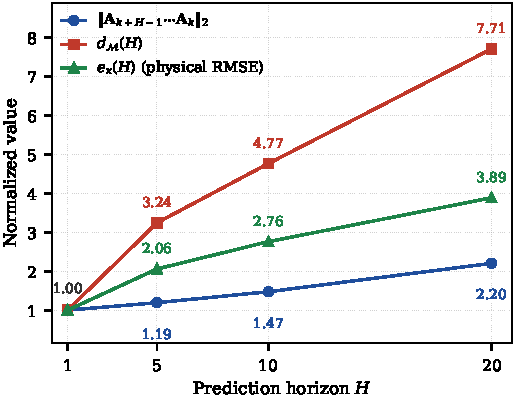
\includegraphics[width=\columnwidth]{pictures/Figure_mechanism.pdf}
\caption{Normalized growth with the prediction horizon $H$ of the finite transition-product norm $\|\mA_{k+H-1}\cdots\mA_k\|_2$, the latent rollout defect $d_{\mathcal M}(H)$, and the physical prediction error $e_x(H)$; each curve is divided by its value at $H=1$ so that different units share one axis. The three quantities grow together with $H$, which is \emph{consistent with} the error-propagation mechanism of Proposition~\ref{prop:propagation}. The figure is an empirical illustration and does not by itself establish a causal chain.}
\label{fig:mechanism}
\end{figure}

Three observations follow, illustrated in Fig.~\ref{fig:mechanism}. First, the transition-product norm grows from $1.05$ to $2.30$ (no contraction) in step with $d_{\mathcal M}$, numerically supporting Remark~\ref{rem:spectral}. Second, the empirical Lipschitz constant is $\widehat{\mLf}\approx1.45>1$, so the finite-horizon form of Theorem~\ref{thm:fh} is the applicable statement and the infinite-horizon limit $\epsilon/(1-\mLf)$ is not available. Third, the Proposition~\ref{prop:propagation} bound is always $\ge$ the actual defect and only $1.64$--$6.52\times$ conservative when compared like-for-like (absolute one-step defects $\epsilon_k$ against absolute rollout defects $d^{\mathrm{abs}}$), and the fitted $\widehat{\mMF}\approx0.007$ is stable across perturbation scales, supporting \eqref{eq:rti_remainder}. The physical-space bound \eqref{eq:cor_physical} is valid but very loose (using $\widehat{\mLf}=1.445$, $53$--$47\,750\times$ over $H=1,\dots,20$), because $\widehat{\mLf}^{H}$ grows geometrically while the true error saturates; we report this honestly rather than presenting the bound as tight.

These measurements bear on the claim that one-step training insufficiently constrains the rollout distribution. That claim rests on the \emph{conjunction} of four observations---a positive one-step consistency defect ($\epsilon_k>0$), a rollout defect $d_{\mathcal M}(H)$ that grows with the horizon, the failure of naive latent propagation, and the recovery obtained under rollout-aware training---and no single observation is sufficient on its own; the latter two are quantified in the experimental study.




% =========================================================
\section{Conclusion}
\label{sec:conclusion}
% =========================================================

This paper presented Transformer-Koopman, a framework for learning history-conditioned Koopman models of controlled nonlinear systems from finite history windows. Because the measured state need not reveal the system's internal dynamics, a patch-based Transformer encoder first maps the history to a structured, state-preserving lifted state. Because a single global lifted transition would then still require all history-dependent regimes to share one evolution law, the lifted transition is additionally modulated by the history through a rank-$r$ term $\mA(\vc)=\mA_0+\mU\,\mathrm{diag}(\gamma_\psi(\vc))\mV^\top$ ($r=2$), which confines history dependence to a structured correction of a shared nominal operator while keeping the propagation conditional-linear. We identified a training--deployment inconsistency between one-step-trained history-conditioned dynamics and the recursively generated latent states seen at deployment, showed that it is not repaired by spectral stabilization, and resolved it with deployment-consistent scheduled training. The rollout-trained scheduled predictor was integrated into a one-iteration RTI-MPC that runs in real time and matches a matched exact scheduled NMPC oracle to within about $1\%$. A finite-horizon theory---finite-history Markovization, latent rollout error propagation, a bounded prediction-error theorem, a physical-space corollary, and a local RTI approximation result---was established and supported by empirical diagnostics. Hardware validation on the soft-robot platform across multi-setpoint, circular, figure-eight, unseen-trajectory, and speed-shift regimes, together with closed-loop baselines against a fixed (time-invariant) Transformer-Koopman controller, remains the immediate next step.

\begin{thebibliography}{99}

\bibitem{koopman1931hamiltonian}
B. O. Koopman, ``Hamiltonian systems and transformation in Hilbert space,'' \emph{Proc. Natl. Acad. Sci. USA}, vol. 17, no. 5, pp. 315--318, 1931.

\bibitem{koopman1932spectra}
B. O. Koopman and J. von Neumann, ``Dynamical systems of continuous spectra,'' \emph{Proc. Natl. Acad. Sci. USA}, vol. 18, no. 3, pp. 255--263, 1932.

\bibitem{mezic2005spectral}
I. Mezi\'c, ``Spectral properties of dynamical systems, model reduction and decompositions,'' \emph{Nonlinear Dyn.}, vol. 41, no. 1--3, pp. 309--325, 2005.

\bibitem{ljung1999system}
L. Ljung, \emph{System Identification: Theory for the User}, 2nd ed. Upper Saddle River, NJ, USA: Prentice Hall PTR, 1999.

\bibitem{vanoverschee1994n4sid}
P. Van Overschee and B. De Moor, ``N4SID: Subspace algorithms for the identification of combined deterministic-stochastic systems,'' \emph{Automatica}, vol. 30, no. 1, pp. 75--93, 1994.

\bibitem{nelles2020nonlinear}
O. Nelles, \emph{Nonlinear System Identification: From Classical Approaches to Neural Networks, Fuzzy Models, and Gaussian Processes}, 2nd ed. Cham, Switzerland: Springer, 2020.

\bibitem{rowley2009spectral}
C. W. Rowley, I. Mezi\'c, S. Bagheri, P. Schlatter, and D. S. Henningson, ``Spectral analysis of nonlinear flows,'' \emph{J. Fluid Mech.}, vol. 641, pp. 115--127, 2009.

\bibitem{williams2015data}
M. O. Williams, I. G. Kevrekidis, and C. W. Rowley, ``A data--driven approximation of the Koopman operator: Extending dynamic mode decomposition,'' \emph{J. Nonlinear Sci.}, vol. 25, no. 6, pp. 1307--1346, 2015.

\bibitem{williams2015kernel}
M. O. Williams, C. W. Rowley, and I. G. Kevrekidis, ``A kernel-based method for data-driven Koopman spectral analysis,'' \emph{J. Comput. Dyn.}, vol. 2, no. 2, pp. 247--265, 2015.

\bibitem{arbabi2017ergodic}
H. Arbabi and I. Mezi\'c, ``Ergodic theory, dynamic mode decomposition, and computation of spectral properties of the Koopman operator,'' \emph{SIAM J. Appl. Dyn. Syst.}, vol. 16, no. 4, pp. 2096--2126, 2017.

\bibitem{kamb2020timedelay}
M. Kamb, E. Kaiser, S. L. Brunton, and J. N. Kutz, ``Time-delay observables for Koopman: Theory and applications,'' \emph{SIAM J. Appl. Dyn. Syst.}, vol. 19, no. 2, pp. 886--917, 2020.

\bibitem{brunton2017chaos}
S. L. Brunton, B. W. Brunton, J. L. Proctor, E. Kaiser, and J. N. Kutz, ``Chaos as an intermittently forced linear system,'' \emph{Nat. Commun.}, vol. 8, art. 19, 2017.

\bibitem{das2019delay}
S. Das and D. Giannakis, ``Delay-coordinate maps and the spectra of Koopman operators,'' \emph{J. Stat. Phys.}, vol. 175, no. 6, pp. 1107--1145, 2019.

\bibitem{liu2023koopa}
Y. Liu, C. Li, J. Wang, and M. Long, ``Koopa: Learning non-stationary time series dynamics with Koopman predictors,'' in \emph{Proc. NeurIPS}, 2023.

\bibitem{li2025mamko}
Z. Li, M. Han, and X. Yin, ``MamKO: Mamba-based Koopman operator for modeling and predictive control,'' in \emph{Proc. ICLR}, 2025.

\bibitem{brunton2022modern}
S. L. Brunton, M. Budi\v{s}i\'c, E. Kaiser, and J. N. Kutz, ``Modern Koopman theory for dynamical systems,'' \emph{SIAM Rev.}, vol. 64, no. 2, pp. 229--340, 2022.

\bibitem{otto2021koopman}
S. E. Otto and C. W. Rowley, ``Koopman operators for estimation and control of dynamical systems,'' \emph{Annu. Rev. Control Robot. Auton. Syst.}, vol. 4, no. 1, pp. 59--87, 2021.

\bibitem{takeishi2017koopman}
N. Takeishi, Y. Kawahara, and T. Yairi, ``Learning Koopman invariant subspaces for dynamic mode decomposition,'' in \emph{Proc. NeurIPS}, 2017, pp. 1130--1140.

\bibitem{yeung2019learning}
E. Yeung, S. Kundu, and N. Hodas, ``Learning deep neural network representations for Koopman operators of nonlinear dynamical systems,'' in \emph{Proc. ACC}, 2019, pp. 4832--4839.

\bibitem{lusch2018deep}
B. Lusch, J. N. Kutz, and S. L. Brunton, ``Deep learning for universal linear embeddings of nonlinear dynamics,'' \emph{Nat. Commun.}, vol. 9, no. 1, p. 4950, 2018.

\bibitem{morton2019deep}
J. Morton, F. D. Witherden, and M. J. Kochenderfer, ``Deep variational Koopman models: Inferring Koopman observations for uncertainty-aware dynamics modeling and control,'' in \emph{Proc. IJCAI}, 2019, pp. 3173--3179.

\bibitem{azencot2020forecasting}
O. Azencot, N. B. Erichson, V. Lin, and M. W. Mahoney, ``Forecasting sequential data using consistent Koopman autoencoders,'' in \emph{Proc. ICML}, 2020, pp. 475--485.

\bibitem{wu2026multistep}
L. Wu, W. G. Y. Tan, L. Zhou, R. D. Braatz, and J. Drgo\v{n}a, ``Least-squares multi-step Koopman operator learning for model predictive control,'' arXiv:2601.11901, 2026.

\bibitem{otto2019linearly}
S. E. Otto and C. W. Rowley, ``Linearly-recurrent autoencoder networks for learning dynamics,'' \emph{SIAM J. Appl. Dyn. Syst.}, vol. 18, no. 1, pp. 558--593, 2019.

\bibitem{forgione2021dynonet}
M. Forgione and D. Piga, ``dynoNet: A neural network architecture for learning dynamical systems,'' \emph{Int. J. Adapt. Control Signal Process.}, vol. 35, no. 4, pp. 612--626, 2021.

\bibitem{proctor2016dmdc}
J. L. Proctor, S. L. Brunton, and J. N. Kutz, ``Dynamic mode decomposition with control,'' \emph{SIAM J. Appl. Dyn. Syst.}, vol. 15, no. 1, pp. 142--161, 2016.

\bibitem{proctor2018generalizing}
J. L. Proctor, S. L. Brunton, and J. N. Kutz, ``Generalizing Koopman theory to allow for inputs and control,'' \emph{SIAM J. Appl. Dyn. Syst.}, vol. 17, no. 1, pp. 909--930, 2018.

\bibitem{brunton2016invariant}
S. L. Brunton, B. W. Brunton, J. L. Proctor, and J. N. Kutz, ``Koopman invariant subspaces and finite linear representations of nonlinear dynamical systems for control,'' \emph{PLOS ONE}, vol. 11, no. 2, e0150171, 2016.

\bibitem{korda2018linear}
M. Korda and I. Mezi\'c, ``Linear predictors for nonlinear dynamical systems: Koopman operator meets model predictive control,'' \emph{Automatica}, vol. 93, pp. 149--160, 2018.

\bibitem{han2020deep}
Y. Han, W. Hao, and U. Vaidya, ``Deep learning of Koopman representation for control,'' in \emph{Proc. IEEE Conf. Decision Control (CDC)}, 2020, pp. 1890--1895.

\bibitem{shi2022deep}
H. Shi and M. Q.-H. Meng, ``Deep Koopman operator with control for nonlinear systems,'' \emph{IEEE Robot. Autom. Lett.}, vol. 7, no. 3, pp. 7700--7707, 2022.

\bibitem{strasser2026overview}
R. Str\"asser, K. Worthmann, I. Mezi\'c, J. Berberich, M. Schaller, and F. Allg\"ower, ``An overview of Koopman-based control: From error bounds to closed-loop guarantees,'' \emph{Annu. Rev. Control}, vol. 61, art. 101035, 2026.

\bibitem{duran2025control}
J. F. Dur\'an-Sig\"uenza, L. I. Minchala, L. E. Garza-Casta\~n\'on, and H. Zhang, ``Control based on the Koopman operator: A comprehensive review,'' \emph{J. Franklin Inst.}, vol. 362, no. 18, art. 108256, 2025.

\bibitem{klus2018data}
S. Klus, F. N\"uske, P. Koltai, H. Wu, I. Kevrekidis, C. Sch\"utte, and F. No\'e, ``Data-driven model reduction and transfer operator approximation,'' \emph{J. Nonlinear Sci.}, vol. 28, no. 3, pp. 985--1010, 2018.

\bibitem{vaswani2017attention}
A. Vaswani \emph{et al.}, ``Attention is all you need,'' in \emph{Proc. NeurIPS}, 2017, pp. 5998--6008.

\bibitem{nie2023time}
Y. Nie, N. H. Nguyen, P. Sinthong, and J. Kalagnanam, ``A time series is worth 64 words: Long-term forecasting with Transformers,'' in \emph{Proc. ICLR}, 2023.

\bibitem{forootani2025deepkoopformer}
A. Forootani, M. Khosravi, and M. Barati, ``DeepKoopFormer: A Koopman enhanced Transformer based architecture for time series forecasting,'' arXiv:2508.02616, 2025.

\bibitem{forootani2026spectral}
A. Forootani and R. Iervolino, ``Learnable Koopman-enhanced Transformer-based time series forecasting with spectral control,'' arXiv:2602.02592, 2026.

\bibitem{feizi2025deepkoopman}
N. Feizi, F. C. Pedrosa, J. Jayender, and R. V. Patel, ``Deep Koopman approach for nonlinear dynamics and control of tendon-driven continuum robots,'' \emph{IEEE Robot. Autom. Lett.}, vol. 10, no. 3, pp. 2926--2933, 2025.

\bibitem{rota1960joint}
G.-C. Rota and G. Strang, ``A note on the joint spectral radius,'' \emph{Nederl. Akad. Wetensch. Proc. Ser. A}, vol. 63 (Indag. Math., vol. 22), pp. 379--381, 1960.

\bibitem{daubechies1992sets}
I. Daubechies and J. C. Lagarias, ``Sets of matrices all infinite products of which converge,'' \emph{Linear Algebra Appl.}, vol. 161, pp. 227--263, 1992.

\bibitem{jungers2009joint}
R. M. Jungers, \emph{The Joint Spectral Radius: Theory and Applications}, Lecture Notes in Control and Information Sciences, vol. 385. Berlin, Germany: Springer, 2009.

\bibitem{diehl2005realtime}
M. Diehl, H. G. Bock, and J. P. Schl\"oder, ``A real-time iteration scheme for nonlinear optimization in optimal feedback control,'' \emph{SIAM J. Control Optim.}, vol. 43, no. 5, pp. 1714--1736, 2005.

\bibitem{gros2020rti}
S. Gros, M. Zanon, R. Quirynen, A. Bemporad, and M. Diehl, ``From linear to nonlinear MPC: Bridging the gap via the real-time iteration,'' \emph{Int. J. Control}, vol. 93, no. 1, pp. 62--80, 2020.

\bibitem{diehl2005rtistability}
M. Diehl, R. Findeisen, F. Allg\"ower, H. G. Bock, and J. P. Schl\"oder, ``Nominal stability of real-time iteration scheme for nonlinear model predictive control,'' \emph{IEE Proc. Control Theory Appl.}, vol. 152, no. 3, pp. 296--308, 2005.

\bibitem{zavala2009advancedstep}
V. M. Zavala and L. T. Biegler, ``The advanced-step NMPC controller: Optimality, stability and robustness,'' \emph{Automatica}, vol. 45, no. 1, pp. 86--93, 2009.

\bibitem{rugh2000gain}
W. J. Rugh and J. S. Shamma, ``Research on gain scheduling,'' \emph{Automatica}, vol. 36, no. 10, pp. 1401--1425, 2000.

\bibitem{leith1998velocity}
D. J. Leith and W. E. Leithead, ``Gain-scheduled and nonlinear systems: Dynamic analysis by velocity-based linearization families,'' \emph{Int. J. Control}, vol. 70, no. 2, pp. 289--317, 1998.

\bibitem{cisneros2016qlmpc}
P. S. G. Cisneros, S. Voss, and H. Werner, ``Efficient nonlinear model predictive control via quasi-LPV representation,'' in \emph{Proc. 55th IEEE Conf. Decision Control (CDC)}, 2016, pp. 3216--3221.

\bibitem{cisneros2020qlpv}
P. S. G. Cisneros and H. Werner, ``Nonlinear model predictive control for models in quasi-linear parameter varying form,'' \emph{Int. J. Robust Nonlinear Control}, vol. 30, no. 10, pp. 3945--3959, 2020.

\end{thebibliography}

\end{document}